% Created by tikzDevice version 0.9 on 2016-01-13 20:58:09
% !TEX encoding = UTF-8 Unicode
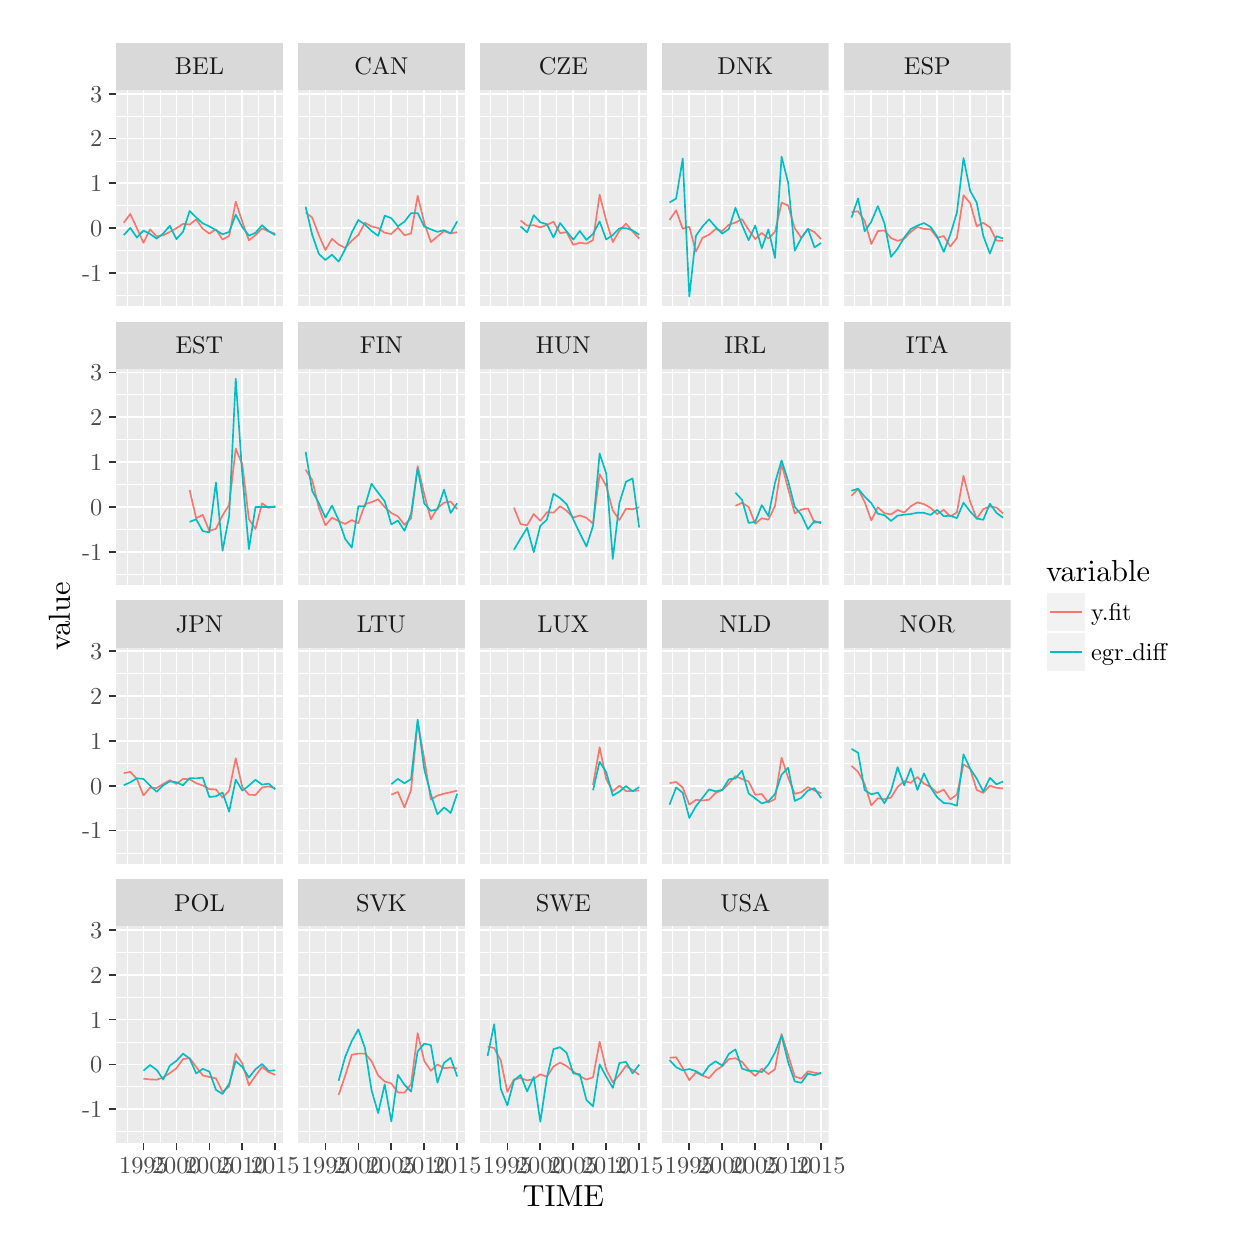
\begin{tikzpicture}[x=1pt,y=1pt]
\definecolor{fillColor}{RGB}{255,255,255}
\path[use as bounding box,fill=fillColor,fill opacity=0.00] (0,0) rectangle (433.62,433.62);
\begin{scope}
\path[clip] (  0.00,  0.00) rectangle (433.62,433.62);
\definecolor{drawColor}{RGB}{255,255,255}
\definecolor{fillColor}{RGB}{255,255,255}

\path[draw=drawColor,line width= 0.6pt,line join=round,line cap=round,fill=fillColor] (  0.00,  0.00) rectangle (433.62,433.62);
\end{scope}
\begin{scope}
\path[clip] ( 31.96,332.89) rectangle ( 92.20,411.06);
\definecolor{fillColor}{gray}{0.92}

\path[fill=fillColor] ( 31.96,332.89) rectangle ( 92.20,411.06);
\definecolor{drawColor}{RGB}{255,255,255}

\path[draw=drawColor,line width= 0.3pt,line join=round] ( 31.96,336.87) --
	( 92.20,336.87);

\path[draw=drawColor,line width= 0.3pt,line join=round] ( 31.96,353.07) --
	( 92.20,353.07);

\path[draw=drawColor,line width= 0.3pt,line join=round] ( 31.96,369.27) --
	( 92.20,369.27);

\path[draw=drawColor,line width= 0.3pt,line join=round] ( 31.96,385.46) --
	( 92.20,385.46);

\path[draw=drawColor,line width= 0.3pt,line join=round] ( 31.96,401.66) --
	( 92.20,401.66);

\path[draw=drawColor,line width= 0.3pt,line join=round] ( 35.89,332.89) --
	( 35.89,411.06);

\path[draw=drawColor,line width= 0.3pt,line join=round] ( 47.79,332.89) --
	( 47.79,411.06);

\path[draw=drawColor,line width= 0.3pt,line join=round] ( 59.70,332.89) --
	( 59.70,411.06);

\path[draw=drawColor,line width= 0.3pt,line join=round] ( 71.61,332.89) --
	( 71.61,411.06);

\path[draw=drawColor,line width= 0.3pt,line join=round] ( 83.51,332.89) --
	( 83.51,411.06);

\path[draw=drawColor,line width= 0.6pt,line join=round] ( 31.96,344.97) --
	( 92.20,344.97);

\path[draw=drawColor,line width= 0.6pt,line join=round] ( 31.96,361.17) --
	( 92.20,361.17);

\path[draw=drawColor,line width= 0.6pt,line join=round] ( 31.96,377.37) --
	( 92.20,377.37);

\path[draw=drawColor,line width= 0.6pt,line join=round] ( 31.96,393.56) --
	( 92.20,393.56);

\path[draw=drawColor,line width= 0.6pt,line join=round] ( 31.96,409.76) --
	( 92.20,409.76);

\path[draw=drawColor,line width= 0.6pt,line join=round] ( 41.84,332.89) --
	( 41.84,411.06);

\path[draw=drawColor,line width= 0.6pt,line join=round] ( 53.75,332.89) --
	( 53.75,411.06);

\path[draw=drawColor,line width= 0.6pt,line join=round] ( 65.65,332.89) --
	( 65.65,411.06);

\path[draw=drawColor,line width= 0.6pt,line join=round] ( 77.56,332.89) --
	( 77.56,411.06);

\path[draw=drawColor,line width= 0.6pt,line join=round] ( 89.47,332.89) --
	( 89.47,411.06);
\definecolor{drawColor}{RGB}{248,118,109}

\path[draw=drawColor,line width= 0.6pt,line join=round] ( 34.70,363.11) --
	( 37.08,366.30) --
	( 39.46,361.19) --
	( 41.84,355.88) --
	( 44.22,360.74) --
	( 46.60,358.18) --
	( 48.98,358.61) --
	( 51.37,359.82) --
	( 53.75,361.15) --
	( 56.13,362.73) --
	( 58.51,362.47) --
	( 60.89,364.34) --
	( 63.27,360.92) --
	( 65.65,359.20) --
	( 68.03,360.75) --
	( 70.42,357.05) --
	( 72.80,358.34) --
	( 75.18,370.75) --
	( 77.56,363.46) --
	( 79.94,356.75) --
	( 82.32,358.63) --
	( 84.70,361.08) --
	( 87.08,359.97) --
	( 89.47,359.15);
\definecolor{drawColor}{RGB}{0,191,196}

\path[draw=drawColor,line width= 0.6pt,line join=round] ( 34.70,358.64) --
	( 37.08,361.25) --
	( 39.46,357.78) --
	( 41.84,360.31) --
	( 44.22,359.08) --
	( 46.60,357.39) --
	( 48.98,359.23) --
	( 51.37,362.05) --
	( 53.75,357.21) --
	( 56.13,359.86) --
	( 58.51,367.38) --
	( 60.89,365.03) --
	( 63.27,362.91) --
	( 65.65,361.81) --
	( 68.03,360.45) --
	( 70.42,358.96) --
	( 72.80,359.79) --
	( 75.18,366.05) --
	( 77.56,361.56) --
	( 79.94,358.45) --
	( 82.32,359.47) --
	( 84.70,362.24) --
	( 87.08,360.07) --
	( 89.47,358.65);
\end{scope}
\begin{scope}
\path[clip] ( 97.70,332.89) rectangle (157.95,411.06);
\definecolor{fillColor}{gray}{0.92}

\path[fill=fillColor] ( 97.70,332.89) rectangle (157.95,411.06);
\definecolor{drawColor}{RGB}{255,255,255}

\path[draw=drawColor,line width= 0.3pt,line join=round] ( 97.70,336.87) --
	(157.95,336.87);

\path[draw=drawColor,line width= 0.3pt,line join=round] ( 97.70,353.07) --
	(157.95,353.07);

\path[draw=drawColor,line width= 0.3pt,line join=round] ( 97.70,369.27) --
	(157.95,369.27);

\path[draw=drawColor,line width= 0.3pt,line join=round] ( 97.70,385.46) --
	(157.95,385.46);

\path[draw=drawColor,line width= 0.3pt,line join=round] ( 97.70,401.66) --
	(157.95,401.66);

\path[draw=drawColor,line width= 0.3pt,line join=round] (101.63,332.89) --
	(101.63,411.06);

\path[draw=drawColor,line width= 0.3pt,line join=round] (113.54,332.89) --
	(113.54,411.06);

\path[draw=drawColor,line width= 0.3pt,line join=round] (125.45,332.89) --
	(125.45,411.06);

\path[draw=drawColor,line width= 0.3pt,line join=round] (137.35,332.89) --
	(137.35,411.06);

\path[draw=drawColor,line width= 0.3pt,line join=round] (149.26,332.89) --
	(149.26,411.06);

\path[draw=drawColor,line width= 0.6pt,line join=round] ( 97.70,344.97) --
	(157.95,344.97);

\path[draw=drawColor,line width= 0.6pt,line join=round] ( 97.70,361.17) --
	(157.95,361.17);

\path[draw=drawColor,line width= 0.6pt,line join=round] ( 97.70,377.37) --
	(157.95,377.37);

\path[draw=drawColor,line width= 0.6pt,line join=round] ( 97.70,393.56) --
	(157.95,393.56);

\path[draw=drawColor,line width= 0.6pt,line join=round] ( 97.70,409.76) --
	(157.95,409.76);

\path[draw=drawColor,line width= 0.6pt,line join=round] (107.59,332.89) --
	(107.59,411.06);

\path[draw=drawColor,line width= 0.6pt,line join=round] (119.49,332.89) --
	(119.49,411.06);

\path[draw=drawColor,line width= 0.6pt,line join=round] (131.40,332.89) --
	(131.40,411.06);

\path[draw=drawColor,line width= 0.6pt,line join=round] (143.31,332.89) --
	(143.31,411.06);

\path[draw=drawColor,line width= 0.6pt,line join=round] (155.21,332.89) --
	(155.21,411.06);
\definecolor{drawColor}{RGB}{248,118,109}

\path[draw=drawColor,line width= 0.6pt,line join=round] (100.44,366.86) --
	(102.82,365.00) --
	(105.21,358.64) --
	(107.59,353.26) --
	(109.97,357.31) --
	(112.35,355.27) --
	(114.73,354.02) --
	(117.11,356.62) --
	(119.49,358.73) --
	(121.87,363.12) --
	(124.26,361.79) --
	(126.64,361.20) --
	(129.02,359.49) --
	(131.40,359.07) --
	(133.78,361.37) --
	(136.16,358.62) --
	(138.54,359.25) --
	(140.92,372.88) --
	(143.31,363.11) --
	(145.69,356.12) --
	(148.07,358.19) --
	(150.45,360.07) --
	(152.83,359.25) --
	(155.21,359.72);
\definecolor{drawColor}{RGB}{0,191,196}

\path[draw=drawColor,line width= 0.6pt,line join=round] (100.44,368.90) --
	(102.82,358.76) --
	(105.21,351.88) --
	(107.59,349.66) --
	(109.97,351.58) --
	(112.35,349.07) --
	(114.73,353.53) --
	(117.11,359.60) --
	(119.49,364.14) --
	(121.87,362.46) --
	(124.26,360.14) --
	(126.64,358.41) --
	(129.02,365.69) --
	(131.40,364.78) --
	(133.78,361.83) --
	(136.16,363.51) --
	(138.54,366.60) --
	(140.92,366.61) --
	(143.31,361.76) --
	(145.69,360.74) --
	(148.07,359.84) --
	(150.45,360.44) --
	(152.83,359.30) --
	(155.21,363.65);
\end{scope}
\begin{scope}
\path[clip] (163.45,332.89) rectangle (223.70,411.06);
\definecolor{fillColor}{gray}{0.92}

\path[fill=fillColor] (163.45,332.89) rectangle (223.70,411.06);
\definecolor{drawColor}{RGB}{255,255,255}

\path[draw=drawColor,line width= 0.3pt,line join=round] (163.45,336.87) --
	(223.70,336.87);

\path[draw=drawColor,line width= 0.3pt,line join=round] (163.45,353.07) --
	(223.70,353.07);

\path[draw=drawColor,line width= 0.3pt,line join=round] (163.45,369.27) --
	(223.70,369.27);

\path[draw=drawColor,line width= 0.3pt,line join=round] (163.45,385.46) --
	(223.70,385.46);

\path[draw=drawColor,line width= 0.3pt,line join=round] (163.45,401.66) --
	(223.70,401.66);

\path[draw=drawColor,line width= 0.3pt,line join=round] (167.38,332.89) --
	(167.38,411.06);

\path[draw=drawColor,line width= 0.3pt,line join=round] (179.29,332.89) --
	(179.29,411.06);

\path[draw=drawColor,line width= 0.3pt,line join=round] (191.19,332.89) --
	(191.19,411.06);

\path[draw=drawColor,line width= 0.3pt,line join=round] (203.10,332.89) --
	(203.10,411.06);

\path[draw=drawColor,line width= 0.3pt,line join=round] (215.01,332.89) --
	(215.01,411.06);

\path[draw=drawColor,line width= 0.6pt,line join=round] (163.45,344.97) --
	(223.70,344.97);

\path[draw=drawColor,line width= 0.6pt,line join=round] (163.45,361.17) --
	(223.70,361.17);

\path[draw=drawColor,line width= 0.6pt,line join=round] (163.45,377.37) --
	(223.70,377.37);

\path[draw=drawColor,line width= 0.6pt,line join=round] (163.45,393.56) --
	(223.70,393.56);

\path[draw=drawColor,line width= 0.6pt,line join=round] (163.45,409.76) --
	(223.70,409.76);

\path[draw=drawColor,line width= 0.6pt,line join=round] (173.33,332.89) --
	(173.33,411.06);

\path[draw=drawColor,line width= 0.6pt,line join=round] (185.24,332.89) --
	(185.24,411.06);

\path[draw=drawColor,line width= 0.6pt,line join=round] (197.15,332.89) --
	(197.15,411.06);

\path[draw=drawColor,line width= 0.6pt,line join=round] (209.05,332.89) --
	(209.05,411.06);

\path[draw=drawColor,line width= 0.6pt,line join=round] (220.96,332.89) --
	(220.96,411.06);
\definecolor{drawColor}{RGB}{248,118,109}

\path[draw=drawColor,line width= 0.6pt,line join=round] (178.10,363.96) --
	(180.48,362.07) --
	(182.86,362.23) --
	(185.24,361.45) --
	(187.62,362.36) --
	(190.00,363.47) --
	(192.38,359.37) --
	(194.76,359.70) --
	(197.15,355.11) --
	(199.53,355.90) --
	(201.91,355.57) --
	(204.29,356.81) --
	(206.67,373.26) --
	(209.05,363.92) --
	(211.43,356.12) --
	(213.81,360.20) --
	(216.20,362.81) --
	(218.58,360.01) --
	(220.96,357.41);
\definecolor{drawColor}{RGB}{0,191,196}

\path[draw=drawColor,line width= 0.6pt,line join=round] (178.10,361.78) --
	(180.48,359.63) --
	(182.86,365.87) --
	(185.24,363.29) --
	(187.62,362.59) --
	(190.00,357.83) --
	(192.38,363.03) --
	(194.76,359.98) --
	(197.15,357.01) --
	(199.53,360.14) --
	(201.91,356.93) --
	(204.29,359.09) --
	(206.67,363.57) --
	(209.05,357.07) --
	(211.43,358.68) --
	(213.81,361.10) --
	(216.20,361.17) --
	(218.58,360.34) --
	(220.96,358.82);
\end{scope}
\begin{scope}
\path[clip] (229.20,332.89) rectangle (289.44,411.06);
\definecolor{fillColor}{gray}{0.92}

\path[fill=fillColor] (229.20,332.89) rectangle (289.44,411.06);
\definecolor{drawColor}{RGB}{255,255,255}

\path[draw=drawColor,line width= 0.3pt,line join=round] (229.20,336.87) --
	(289.44,336.87);

\path[draw=drawColor,line width= 0.3pt,line join=round] (229.20,353.07) --
	(289.44,353.07);

\path[draw=drawColor,line width= 0.3pt,line join=round] (229.20,369.27) --
	(289.44,369.27);

\path[draw=drawColor,line width= 0.3pt,line join=round] (229.20,385.46) --
	(289.44,385.46);

\path[draw=drawColor,line width= 0.3pt,line join=round] (229.20,401.66) --
	(289.44,401.66);

\path[draw=drawColor,line width= 0.3pt,line join=round] (233.13,332.89) --
	(233.13,411.06);

\path[draw=drawColor,line width= 0.3pt,line join=round] (245.03,332.89) --
	(245.03,411.06);

\path[draw=drawColor,line width= 0.3pt,line join=round] (256.94,332.89) --
	(256.94,411.06);

\path[draw=drawColor,line width= 0.3pt,line join=round] (268.85,332.89) --
	(268.85,411.06);

\path[draw=drawColor,line width= 0.3pt,line join=round] (280.75,332.89) --
	(280.75,411.06);

\path[draw=drawColor,line width= 0.6pt,line join=round] (229.20,344.97) --
	(289.44,344.97);

\path[draw=drawColor,line width= 0.6pt,line join=round] (229.20,361.17) --
	(289.44,361.17);

\path[draw=drawColor,line width= 0.6pt,line join=round] (229.20,377.37) --
	(289.44,377.37);

\path[draw=drawColor,line width= 0.6pt,line join=round] (229.20,393.56) --
	(289.44,393.56);

\path[draw=drawColor,line width= 0.6pt,line join=round] (229.20,409.76) --
	(289.44,409.76);

\path[draw=drawColor,line width= 0.6pt,line join=round] (239.08,332.89) --
	(239.08,411.06);

\path[draw=drawColor,line width= 0.6pt,line join=round] (250.99,332.89) --
	(250.99,411.06);

\path[draw=drawColor,line width= 0.6pt,line join=round] (262.89,332.89) --
	(262.89,411.06);

\path[draw=drawColor,line width= 0.6pt,line join=round] (274.80,332.89) --
	(274.80,411.06);

\path[draw=drawColor,line width= 0.6pt,line join=round] (286.71,332.89) --
	(286.71,411.06);
\definecolor{drawColor}{RGB}{248,118,109}

\path[draw=drawColor,line width= 0.6pt,line join=round] (231.94,364.13) --
	(234.32,367.64) --
	(236.70,360.93) --
	(239.08,361.66) --
	(241.46,352.69) --
	(243.84,357.67) --
	(246.22,358.81) --
	(248.60,360.86) --
	(250.99,360.13) --
	(253.37,362.40) --
	(255.75,363.22) --
	(258.13,364.42) --
	(260.51,360.58) --
	(262.89,357.23) --
	(265.27,359.46) --
	(267.65,357.39) --
	(270.04,359.86) --
	(272.42,370.38) --
	(274.80,369.34) --
	(277.18,361.12) --
	(279.56,357.65) --
	(281.94,360.92) --
	(284.32,359.72) --
	(286.71,357.19);
\definecolor{drawColor}{RGB}{0,191,196}

\path[draw=drawColor,line width= 0.6pt,line join=round] (231.94,370.43) --
	(234.32,371.86) --
	(236.70,386.33) --
	(239.08,336.44) --
	(241.46,358.39) --
	(243.84,361.79) --
	(246.22,364.36) --
	(248.60,361.57) --
	(250.99,359.18) --
	(253.37,360.87) --
	(255.75,368.53) --
	(258.13,362.29) --
	(260.51,356.83) --
	(262.89,362.11) --
	(265.27,353.94) --
	(267.65,360.73) --
	(270.04,350.41) --
	(272.42,387.03) --
	(274.80,377.55) --
	(277.18,353.01) --
	(279.56,357.60) --
	(281.94,360.92) --
	(284.32,354.24) --
	(286.71,355.82);
\end{scope}
\begin{scope}
\path[clip] (294.94,332.89) rectangle (355.19,411.06);
\definecolor{fillColor}{gray}{0.92}

\path[fill=fillColor] (294.94,332.89) rectangle (355.19,411.06);
\definecolor{drawColor}{RGB}{255,255,255}

\path[draw=drawColor,line width= 0.3pt,line join=round] (294.94,336.87) --
	(355.19,336.87);

\path[draw=drawColor,line width= 0.3pt,line join=round] (294.94,353.07) --
	(355.19,353.07);

\path[draw=drawColor,line width= 0.3pt,line join=round] (294.94,369.27) --
	(355.19,369.27);

\path[draw=drawColor,line width= 0.3pt,line join=round] (294.94,385.46) --
	(355.19,385.46);

\path[draw=drawColor,line width= 0.3pt,line join=round] (294.94,401.66) --
	(355.19,401.66);

\path[draw=drawColor,line width= 0.3pt,line join=round] (298.87,332.89) --
	(298.87,411.06);

\path[draw=drawColor,line width= 0.3pt,line join=round] (310.78,332.89) --
	(310.78,411.06);

\path[draw=drawColor,line width= 0.3pt,line join=round] (322.69,332.89) --
	(322.69,411.06);

\path[draw=drawColor,line width= 0.3pt,line join=round] (334.59,332.89) --
	(334.59,411.06);

\path[draw=drawColor,line width= 0.3pt,line join=round] (346.50,332.89) --
	(346.50,411.06);

\path[draw=drawColor,line width= 0.6pt,line join=round] (294.94,344.97) --
	(355.19,344.97);

\path[draw=drawColor,line width= 0.6pt,line join=round] (294.94,361.17) --
	(355.19,361.17);

\path[draw=drawColor,line width= 0.6pt,line join=round] (294.94,377.37) --
	(355.19,377.37);

\path[draw=drawColor,line width= 0.6pt,line join=round] (294.94,393.56) --
	(355.19,393.56);

\path[draw=drawColor,line width= 0.6pt,line join=round] (294.94,409.76) --
	(355.19,409.76);

\path[draw=drawColor,line width= 0.6pt,line join=round] (304.83,332.89) --
	(304.83,411.06);

\path[draw=drawColor,line width= 0.6pt,line join=round] (316.73,332.89) --
	(316.73,411.06);

\path[draw=drawColor,line width= 0.6pt,line join=round] (328.64,332.89) --
	(328.64,411.06);

\path[draw=drawColor,line width= 0.6pt,line join=round] (340.55,332.89) --
	(340.55,411.06);

\path[draw=drawColor,line width= 0.6pt,line join=round] (352.45,332.89) --
	(352.45,411.06);
\definecolor{drawColor}{RGB}{248,118,109}

\path[draw=drawColor,line width= 0.6pt,line join=round] (297.68,366.96) --
	(300.06,367.26) --
	(302.44,363.80) --
	(304.83,355.43) --
	(307.21,360.12) --
	(309.59,360.35) --
	(311.97,357.58) --
	(314.35,356.59) --
	(316.73,357.35) --
	(319.11,359.83) --
	(321.50,361.60) --
	(323.88,360.89) --
	(326.26,360.77) --
	(328.64,357.69) --
	(331.02,358.33) --
	(333.40,354.55) --
	(335.78,357.64) --
	(338.16,373.05) --
	(340.55,370.27) --
	(342.93,361.85) --
	(345.31,363.12) --
	(347.69,361.50) --
	(350.07,356.67) --
	(352.45,356.58);
\definecolor{drawColor}{RGB}{0,191,196}

\path[draw=drawColor,line width= 0.6pt,line join=round] (297.68,364.98) --
	(300.06,371.94) --
	(302.44,360.04) --
	(304.83,363.47) --
	(307.21,369.17) --
	(309.59,362.89) --
	(311.97,350.78) --
	(314.35,353.77) --
	(316.73,357.78) --
	(319.11,360.88) --
	(321.50,362.10) --
	(323.88,363.01) --
	(326.26,361.63) --
	(328.64,358.18) --
	(331.02,352.59) --
	(333.40,358.92) --
	(335.78,366.83) --
	(338.16,386.49) --
	(340.55,374.68) --
	(342.93,370.41) --
	(345.31,358.37) --
	(347.69,351.99) --
	(350.07,358.25) --
	(352.45,357.46);
\end{scope}
\begin{scope}
\path[clip] ( 31.96,232.15) rectangle ( 92.20,310.33);
\definecolor{fillColor}{gray}{0.92}

\path[fill=fillColor] ( 31.96,232.15) rectangle ( 92.20,310.33);
\definecolor{drawColor}{RGB}{255,255,255}

\path[draw=drawColor,line width= 0.3pt,line join=round] ( 31.96,236.14) --
	( 92.20,236.14);

\path[draw=drawColor,line width= 0.3pt,line join=round] ( 31.96,252.34) --
	( 92.20,252.34);

\path[draw=drawColor,line width= 0.3pt,line join=round] ( 31.96,268.53) --
	( 92.20,268.53);

\path[draw=drawColor,line width= 0.3pt,line join=round] ( 31.96,284.73) --
	( 92.20,284.73);

\path[draw=drawColor,line width= 0.3pt,line join=round] ( 31.96,300.93) --
	( 92.20,300.93);

\path[draw=drawColor,line width= 0.3pt,line join=round] ( 35.89,232.15) --
	( 35.89,310.33);

\path[draw=drawColor,line width= 0.3pt,line join=round] ( 47.79,232.15) --
	( 47.79,310.33);

\path[draw=drawColor,line width= 0.3pt,line join=round] ( 59.70,232.15) --
	( 59.70,310.33);

\path[draw=drawColor,line width= 0.3pt,line join=round] ( 71.61,232.15) --
	( 71.61,310.33);

\path[draw=drawColor,line width= 0.3pt,line join=round] ( 83.51,232.15) --
	( 83.51,310.33);

\path[draw=drawColor,line width= 0.6pt,line join=round] ( 31.96,244.24) --
	( 92.20,244.24);

\path[draw=drawColor,line width= 0.6pt,line join=round] ( 31.96,260.44) --
	( 92.20,260.44);

\path[draw=drawColor,line width= 0.6pt,line join=round] ( 31.96,276.63) --
	( 92.20,276.63);

\path[draw=drawColor,line width= 0.6pt,line join=round] ( 31.96,292.83) --
	( 92.20,292.83);

\path[draw=drawColor,line width= 0.6pt,line join=round] ( 31.96,309.03) --
	( 92.20,309.03);

\path[draw=drawColor,line width= 0.6pt,line join=round] ( 41.84,232.15) --
	( 41.84,310.33);

\path[draw=drawColor,line width= 0.6pt,line join=round] ( 53.75,232.15) --
	( 53.75,310.33);

\path[draw=drawColor,line width= 0.6pt,line join=round] ( 65.65,232.15) --
	( 65.65,310.33);

\path[draw=drawColor,line width= 0.6pt,line join=round] ( 77.56,232.15) --
	( 77.56,310.33);

\path[draw=drawColor,line width= 0.6pt,line join=round] ( 89.47,232.15) --
	( 89.47,310.33);
\definecolor{drawColor}{RGB}{248,118,109}

\path[draw=drawColor,line width= 0.6pt,line join=round] ( 58.51,266.55) --
	( 60.89,256.33) --
	( 63.27,257.57) --
	( 65.65,251.74) --
	( 68.03,252.53) --
	( 70.42,257.38) --
	( 72.80,261.18) --
	( 75.18,281.54) --
	( 77.56,275.75) --
	( 79.94,256.00) --
	( 82.32,252.50) --
	( 84.70,261.74) --
	( 87.08,260.11) --
	( 89.47,260.72);
\definecolor{drawColor}{RGB}{0,191,196}

\path[draw=drawColor,line width= 0.6pt,line join=round] ( 58.51,255.04) --
	( 60.89,255.97) --
	( 63.27,251.67) --
	( 65.65,251.25) --
	( 68.03,269.27) --
	( 70.42,244.68) --
	( 72.80,257.10) --
	( 75.18,306.77) --
	( 77.56,271.92) --
	( 79.94,245.17) --
	( 82.32,260.44) --
	( 84.70,260.44) --
	( 87.08,260.44) --
	( 89.47,260.44);
\end{scope}
\begin{scope}
\path[clip] ( 97.70,232.15) rectangle (157.95,310.33);
\definecolor{fillColor}{gray}{0.92}

\path[fill=fillColor] ( 97.70,232.15) rectangle (157.95,310.33);
\definecolor{drawColor}{RGB}{255,255,255}

\path[draw=drawColor,line width= 0.3pt,line join=round] ( 97.70,236.14) --
	(157.95,236.14);

\path[draw=drawColor,line width= 0.3pt,line join=round] ( 97.70,252.34) --
	(157.95,252.34);

\path[draw=drawColor,line width= 0.3pt,line join=round] ( 97.70,268.53) --
	(157.95,268.53);

\path[draw=drawColor,line width= 0.3pt,line join=round] ( 97.70,284.73) --
	(157.95,284.73);

\path[draw=drawColor,line width= 0.3pt,line join=round] ( 97.70,300.93) --
	(157.95,300.93);

\path[draw=drawColor,line width= 0.3pt,line join=round] (101.63,232.15) --
	(101.63,310.33);

\path[draw=drawColor,line width= 0.3pt,line join=round] (113.54,232.15) --
	(113.54,310.33);

\path[draw=drawColor,line width= 0.3pt,line join=round] (125.45,232.15) --
	(125.45,310.33);

\path[draw=drawColor,line width= 0.3pt,line join=round] (137.35,232.15) --
	(137.35,310.33);

\path[draw=drawColor,line width= 0.3pt,line join=round] (149.26,232.15) --
	(149.26,310.33);

\path[draw=drawColor,line width= 0.6pt,line join=round] ( 97.70,244.24) --
	(157.95,244.24);

\path[draw=drawColor,line width= 0.6pt,line join=round] ( 97.70,260.44) --
	(157.95,260.44);

\path[draw=drawColor,line width= 0.6pt,line join=round] ( 97.70,276.63) --
	(157.95,276.63);

\path[draw=drawColor,line width= 0.6pt,line join=round] ( 97.70,292.83) --
	(157.95,292.83);

\path[draw=drawColor,line width= 0.6pt,line join=round] ( 97.70,309.03) --
	(157.95,309.03);

\path[draw=drawColor,line width= 0.6pt,line join=round] (107.59,232.15) --
	(107.59,310.33);

\path[draw=drawColor,line width= 0.6pt,line join=round] (119.49,232.15) --
	(119.49,310.33);

\path[draw=drawColor,line width= 0.6pt,line join=round] (131.40,232.15) --
	(131.40,310.33);

\path[draw=drawColor,line width= 0.6pt,line join=round] (143.31,232.15) --
	(143.31,310.33);

\path[draw=drawColor,line width= 0.6pt,line join=round] (155.21,232.15) --
	(155.21,310.33);
\definecolor{drawColor}{RGB}{248,118,109}

\path[draw=drawColor,line width= 0.6pt,line join=round] (100.44,273.88) --
	(102.82,270.14) --
	(105.21,260.14) --
	(107.59,253.76) --
	(109.97,256.55) --
	(112.35,255.33) --
	(114.73,254.30) --
	(117.11,255.69) --
	(119.49,254.55) --
	(121.87,261.39) --
	(124.26,262.18) --
	(126.64,263.18) --
	(129.02,260.36) --
	(131.40,258.26) --
	(133.78,257.04) --
	(136.16,253.94) --
	(138.54,256.31) --
	(140.92,275.17) --
	(143.31,265.02) --
	(145.69,255.95) --
	(148.07,260.04) --
	(150.45,261.94) --
	(152.83,262.38) --
	(155.21,259.62);
\definecolor{drawColor}{RGB}{0,191,196}

\path[draw=drawColor,line width= 0.6pt,line join=round] (100.44,280.35) --
	(102.82,266.20) --
	(105.21,261.84) --
	(107.59,256.57) --
	(109.97,260.91) --
	(112.35,255.73) --
	(114.73,248.88) --
	(117.11,245.73) --
	(119.49,260.71) --
	(121.87,260.70) --
	(124.26,268.82) --
	(126.64,265.56) --
	(129.02,262.49) --
	(131.40,254.12) --
	(133.78,255.52) --
	(136.16,251.84) --
	(138.54,257.99) --
	(140.92,274.30) --
	(143.31,261.65) --
	(145.69,259.03) --
	(148.07,259.57) --
	(150.45,266.69) --
	(152.83,258.25) --
	(155.21,261.76);
\end{scope}
\begin{scope}
\path[clip] (163.45,232.15) rectangle (223.70,310.33);
\definecolor{fillColor}{gray}{0.92}

\path[fill=fillColor] (163.45,232.15) rectangle (223.70,310.33);
\definecolor{drawColor}{RGB}{255,255,255}

\path[draw=drawColor,line width= 0.3pt,line join=round] (163.45,236.14) --
	(223.70,236.14);

\path[draw=drawColor,line width= 0.3pt,line join=round] (163.45,252.34) --
	(223.70,252.34);

\path[draw=drawColor,line width= 0.3pt,line join=round] (163.45,268.53) --
	(223.70,268.53);

\path[draw=drawColor,line width= 0.3pt,line join=round] (163.45,284.73) --
	(223.70,284.73);

\path[draw=drawColor,line width= 0.3pt,line join=round] (163.45,300.93) --
	(223.70,300.93);

\path[draw=drawColor,line width= 0.3pt,line join=round] (167.38,232.15) --
	(167.38,310.33);

\path[draw=drawColor,line width= 0.3pt,line join=round] (179.29,232.15) --
	(179.29,310.33);

\path[draw=drawColor,line width= 0.3pt,line join=round] (191.19,232.15) --
	(191.19,310.33);

\path[draw=drawColor,line width= 0.3pt,line join=round] (203.10,232.15) --
	(203.10,310.33);

\path[draw=drawColor,line width= 0.3pt,line join=round] (215.01,232.15) --
	(215.01,310.33);

\path[draw=drawColor,line width= 0.6pt,line join=round] (163.45,244.24) --
	(223.70,244.24);

\path[draw=drawColor,line width= 0.6pt,line join=round] (163.45,260.44) --
	(223.70,260.44);

\path[draw=drawColor,line width= 0.6pt,line join=round] (163.45,276.63) --
	(223.70,276.63);

\path[draw=drawColor,line width= 0.6pt,line join=round] (163.45,292.83) --
	(223.70,292.83);

\path[draw=drawColor,line width= 0.6pt,line join=round] (163.45,309.03) --
	(223.70,309.03);

\path[draw=drawColor,line width= 0.6pt,line join=round] (173.33,232.15) --
	(173.33,310.33);

\path[draw=drawColor,line width= 0.6pt,line join=round] (185.24,232.15) --
	(185.24,310.33);

\path[draw=drawColor,line width= 0.6pt,line join=round] (197.15,232.15) --
	(197.15,310.33);

\path[draw=drawColor,line width= 0.6pt,line join=round] (209.05,232.15) --
	(209.05,310.33);

\path[draw=drawColor,line width= 0.6pt,line join=round] (220.96,232.15) --
	(220.96,310.33);
\definecolor{drawColor}{RGB}{248,118,109}

\path[draw=drawColor,line width= 0.6pt,line join=round] (175.71,260.18) --
	(178.10,254.24) --
	(180.48,253.81) --
	(182.86,257.88) --
	(185.24,255.40) --
	(187.62,258.51) --
	(190.00,258.36) --
	(192.38,260.69) --
	(194.76,259.04) --
	(197.15,256.55) --
	(199.53,257.37) --
	(201.91,256.50) --
	(204.29,254.36) --
	(206.67,272.29) --
	(209.05,268.06) --
	(211.43,259.18) --
	(213.81,255.71) --
	(216.20,259.78) --
	(218.58,259.60) --
	(220.96,260.32);
\definecolor{drawColor}{RGB}{0,191,196}

\path[draw=drawColor,line width= 0.6pt,line join=round] (175.71,244.94) --
	(178.10,249.00) --
	(180.48,252.88) --
	(182.86,244.09) --
	(185.24,253.60) --
	(187.62,255.83) --
	(190.00,265.19) --
	(192.38,263.63) --
	(194.76,261.41) --
	(197.15,255.93) --
	(199.53,250.90) --
	(201.91,246.14) --
	(204.29,253.60) --
	(206.67,279.73) --
	(209.05,272.54) --
	(211.43,241.65) --
	(213.81,261.85) --
	(216.20,269.54) --
	(218.58,270.74) --
	(220.96,252.98);
\end{scope}
\begin{scope}
\path[clip] (229.20,232.15) rectangle (289.44,310.33);
\definecolor{fillColor}{gray}{0.92}

\path[fill=fillColor] (229.20,232.15) rectangle (289.44,310.33);
\definecolor{drawColor}{RGB}{255,255,255}

\path[draw=drawColor,line width= 0.3pt,line join=round] (229.20,236.14) --
	(289.44,236.14);

\path[draw=drawColor,line width= 0.3pt,line join=round] (229.20,252.34) --
	(289.44,252.34);

\path[draw=drawColor,line width= 0.3pt,line join=round] (229.20,268.53) --
	(289.44,268.53);

\path[draw=drawColor,line width= 0.3pt,line join=round] (229.20,284.73) --
	(289.44,284.73);

\path[draw=drawColor,line width= 0.3pt,line join=round] (229.20,300.93) --
	(289.44,300.93);

\path[draw=drawColor,line width= 0.3pt,line join=round] (233.13,232.15) --
	(233.13,310.33);

\path[draw=drawColor,line width= 0.3pt,line join=round] (245.03,232.15) --
	(245.03,310.33);

\path[draw=drawColor,line width= 0.3pt,line join=round] (256.94,232.15) --
	(256.94,310.33);

\path[draw=drawColor,line width= 0.3pt,line join=round] (268.85,232.15) --
	(268.85,310.33);

\path[draw=drawColor,line width= 0.3pt,line join=round] (280.75,232.15) --
	(280.75,310.33);

\path[draw=drawColor,line width= 0.6pt,line join=round] (229.20,244.24) --
	(289.44,244.24);

\path[draw=drawColor,line width= 0.6pt,line join=round] (229.20,260.44) --
	(289.44,260.44);

\path[draw=drawColor,line width= 0.6pt,line join=round] (229.20,276.63) --
	(289.44,276.63);

\path[draw=drawColor,line width= 0.6pt,line join=round] (229.20,292.83) --
	(289.44,292.83);

\path[draw=drawColor,line width= 0.6pt,line join=round] (229.20,309.03) --
	(289.44,309.03);

\path[draw=drawColor,line width= 0.6pt,line join=round] (239.08,232.15) --
	(239.08,310.33);

\path[draw=drawColor,line width= 0.6pt,line join=round] (250.99,232.15) --
	(250.99,310.33);

\path[draw=drawColor,line width= 0.6pt,line join=round] (262.89,232.15) --
	(262.89,310.33);

\path[draw=drawColor,line width= 0.6pt,line join=round] (274.80,232.15) --
	(274.80,310.33);

\path[draw=drawColor,line width= 0.6pt,line join=round] (286.71,232.15) --
	(286.71,310.33);
\definecolor{drawColor}{RGB}{248,118,109}

\path[draw=drawColor,line width= 0.6pt,line join=round] (255.75,260.83) --
	(258.13,261.94) --
	(260.51,260.44) --
	(262.89,254.36) --
	(265.27,256.34) --
	(267.65,255.84) --
	(270.04,260.76) --
	(272.42,276.08) --
	(274.80,266.91) --
	(277.18,258.11) --
	(279.56,259.48) --
	(281.94,259.92) --
	(284.32,254.73) --
	(286.71,255.05);
\definecolor{drawColor}{RGB}{0,191,196}

\path[draw=drawColor,line width= 0.6pt,line join=round] (255.75,265.58) --
	(258.13,262.98) --
	(260.51,254.66) --
	(262.89,255.04) --
	(265.27,261.11) --
	(267.65,257.16) --
	(270.04,269.16) --
	(272.42,277.25) --
	(274.80,269.76) --
	(277.18,260.45) --
	(279.56,257.59) --
	(281.94,252.41) --
	(284.32,255.36) --
	(286.71,254.51);
\end{scope}
\begin{scope}
\path[clip] (294.94,232.15) rectangle (355.19,310.33);
\definecolor{fillColor}{gray}{0.92}

\path[fill=fillColor] (294.94,232.15) rectangle (355.19,310.33);
\definecolor{drawColor}{RGB}{255,255,255}

\path[draw=drawColor,line width= 0.3pt,line join=round] (294.94,236.14) --
	(355.19,236.14);

\path[draw=drawColor,line width= 0.3pt,line join=round] (294.94,252.34) --
	(355.19,252.34);

\path[draw=drawColor,line width= 0.3pt,line join=round] (294.94,268.53) --
	(355.19,268.53);

\path[draw=drawColor,line width= 0.3pt,line join=round] (294.94,284.73) --
	(355.19,284.73);

\path[draw=drawColor,line width= 0.3pt,line join=round] (294.94,300.93) --
	(355.19,300.93);

\path[draw=drawColor,line width= 0.3pt,line join=round] (298.87,232.15) --
	(298.87,310.33);

\path[draw=drawColor,line width= 0.3pt,line join=round] (310.78,232.15) --
	(310.78,310.33);

\path[draw=drawColor,line width= 0.3pt,line join=round] (322.69,232.15) --
	(322.69,310.33);

\path[draw=drawColor,line width= 0.3pt,line join=round] (334.59,232.15) --
	(334.59,310.33);

\path[draw=drawColor,line width= 0.3pt,line join=round] (346.50,232.15) --
	(346.50,310.33);

\path[draw=drawColor,line width= 0.6pt,line join=round] (294.94,244.24) --
	(355.19,244.24);

\path[draw=drawColor,line width= 0.6pt,line join=round] (294.94,260.44) --
	(355.19,260.44);

\path[draw=drawColor,line width= 0.6pt,line join=round] (294.94,276.63) --
	(355.19,276.63);

\path[draw=drawColor,line width= 0.6pt,line join=round] (294.94,292.83) --
	(355.19,292.83);

\path[draw=drawColor,line width= 0.6pt,line join=round] (294.94,309.03) --
	(355.19,309.03);

\path[draw=drawColor,line width= 0.6pt,line join=round] (304.83,232.15) --
	(304.83,310.33);

\path[draw=drawColor,line width= 0.6pt,line join=round] (316.73,232.15) --
	(316.73,310.33);

\path[draw=drawColor,line width= 0.6pt,line join=round] (328.64,232.15) --
	(328.64,310.33);

\path[draw=drawColor,line width= 0.6pt,line join=round] (340.55,232.15) --
	(340.55,310.33);

\path[draw=drawColor,line width= 0.6pt,line join=round] (352.45,232.15) --
	(352.45,310.33);
\definecolor{drawColor}{RGB}{248,118,109}

\path[draw=drawColor,line width= 0.6pt,line join=round] (297.68,264.47) --
	(300.06,266.90) --
	(302.44,262.24) --
	(304.83,255.56) --
	(307.21,260.31) --
	(309.59,258.16) --
	(311.97,257.72) --
	(314.35,259.34) --
	(316.73,258.39) --
	(319.11,260.69) --
	(321.50,262.09) --
	(323.88,261.44) --
	(326.26,260.11) --
	(328.64,257.84) --
	(331.02,259.40) --
	(333.40,256.97) --
	(335.78,258.47) --
	(338.16,271.68) --
	(340.55,262.31) --
	(342.93,256.15) --
	(345.31,259.65) --
	(347.69,260.63) --
	(350.07,260.21) --
	(352.45,258.10);
\definecolor{drawColor}{RGB}{0,191,196}

\path[draw=drawColor,line width= 0.6pt,line join=round] (297.68,266.27) --
	(300.06,267.05) --
	(302.44,264.15) --
	(304.83,261.83) --
	(307.21,258.00) --
	(309.59,257.44) --
	(311.97,255.39) --
	(314.35,257.28) --
	(316.73,257.64) --
	(319.11,257.87) --
	(321.50,258.34) --
	(323.88,258.30) --
	(326.26,257.55) --
	(328.64,259.37) --
	(331.02,257.09) --
	(333.40,257.28) --
	(335.78,256.39) --
	(338.16,261.98) --
	(340.55,258.81) --
	(342.93,256.25) --
	(345.31,255.80) --
	(347.69,261.61) --
	(350.07,258.30) --
	(352.45,256.53);
\end{scope}
\begin{scope}
\path[clip] ( 31.96,131.42) rectangle ( 92.20,209.59);
\definecolor{fillColor}{gray}{0.92}

\path[fill=fillColor] ( 31.96,131.42) rectangle ( 92.20,209.59);
\definecolor{drawColor}{RGB}{255,255,255}

\path[draw=drawColor,line width= 0.3pt,line join=round] ( 31.96,135.41) --
	( 92.20,135.41);

\path[draw=drawColor,line width= 0.3pt,line join=round] ( 31.96,151.60) --
	( 92.20,151.60);

\path[draw=drawColor,line width= 0.3pt,line join=round] ( 31.96,167.80) --
	( 92.20,167.80);

\path[draw=drawColor,line width= 0.3pt,line join=round] ( 31.96,184.00) --
	( 92.20,184.00);

\path[draw=drawColor,line width= 0.3pt,line join=round] ( 31.96,200.20) --
	( 92.20,200.20);

\path[draw=drawColor,line width= 0.3pt,line join=round] ( 35.89,131.42) --
	( 35.89,209.59);

\path[draw=drawColor,line width= 0.3pt,line join=round] ( 47.79,131.42) --
	( 47.79,209.59);

\path[draw=drawColor,line width= 0.3pt,line join=round] ( 59.70,131.42) --
	( 59.70,209.59);

\path[draw=drawColor,line width= 0.3pt,line join=round] ( 71.61,131.42) --
	( 71.61,209.59);

\path[draw=drawColor,line width= 0.3pt,line join=round] ( 83.51,131.42) --
	( 83.51,209.59);

\path[draw=drawColor,line width= 0.6pt,line join=round] ( 31.96,143.51) --
	( 92.20,143.51);

\path[draw=drawColor,line width= 0.6pt,line join=round] ( 31.96,159.70) --
	( 92.20,159.70);

\path[draw=drawColor,line width= 0.6pt,line join=round] ( 31.96,175.90) --
	( 92.20,175.90);

\path[draw=drawColor,line width= 0.6pt,line join=round] ( 31.96,192.10) --
	( 92.20,192.10);

\path[draw=drawColor,line width= 0.6pt,line join=round] ( 31.96,208.29) --
	( 92.20,208.29);

\path[draw=drawColor,line width= 0.6pt,line join=round] ( 41.84,131.42) --
	( 41.84,209.59);

\path[draw=drawColor,line width= 0.6pt,line join=round] ( 53.75,131.42) --
	( 53.75,209.59);

\path[draw=drawColor,line width= 0.6pt,line join=round] ( 65.65,131.42) --
	( 65.65,209.59);

\path[draw=drawColor,line width= 0.6pt,line join=round] ( 77.56,131.42) --
	( 77.56,209.59);

\path[draw=drawColor,line width= 0.6pt,line join=round] ( 89.47,131.42) --
	( 89.47,209.59);
\definecolor{drawColor}{RGB}{248,118,109}

\path[draw=drawColor,line width= 0.6pt,line join=round] ( 34.70,164.24) --
	( 37.08,164.71) --
	( 39.46,162.16) --
	( 41.84,156.17) --
	( 44.22,158.98) --
	( 46.60,158.88) --
	( 48.98,160.35) --
	( 51.37,161.69) --
	( 53.75,160.33) --
	( 56.13,162.18) --
	( 58.51,162.01) --
	( 60.89,160.63) --
	( 63.27,159.78) --
	( 65.65,158.49) --
	( 68.03,158.34) --
	( 70.42,155.40) --
	( 72.80,157.93) --
	( 75.18,169.63) --
	( 77.56,159.19) --
	( 79.94,156.45) --
	( 82.32,156.33) --
	( 84.70,159.07) --
	( 87.08,159.45) --
	( 89.47,158.74);
\definecolor{drawColor}{RGB}{0,191,196}

\path[draw=drawColor,line width= 0.6pt,line join=round] ( 34.70,159.85) --
	( 37.08,160.93) --
	( 39.46,162.39) --
	( 41.84,162.13) --
	( 44.22,159.74) --
	( 46.60,157.50) --
	( 48.98,159.83) --
	( 51.37,161.28) --
	( 53.75,160.94) --
	( 56.13,159.89) --
	( 58.51,162.41) --
	( 60.89,162.35) --
	( 63.27,162.64) --
	( 65.65,155.62) --
	( 68.03,155.89) --
	( 70.42,157.24) --
	( 72.80,150.32) --
	( 75.18,161.90) --
	( 77.56,157.93) --
	( 79.94,159.76) --
	( 82.32,161.84) --
	( 84.70,160.08) --
	( 87.08,160.46) --
	( 89.47,158.37);
\end{scope}
\begin{scope}
\path[clip] ( 97.70,131.42) rectangle (157.95,209.59);
\definecolor{fillColor}{gray}{0.92}

\path[fill=fillColor] ( 97.70,131.42) rectangle (157.95,209.59);
\definecolor{drawColor}{RGB}{255,255,255}

\path[draw=drawColor,line width= 0.3pt,line join=round] ( 97.70,135.41) --
	(157.95,135.41);

\path[draw=drawColor,line width= 0.3pt,line join=round] ( 97.70,151.60) --
	(157.95,151.60);

\path[draw=drawColor,line width= 0.3pt,line join=round] ( 97.70,167.80) --
	(157.95,167.80);

\path[draw=drawColor,line width= 0.3pt,line join=round] ( 97.70,184.00) --
	(157.95,184.00);

\path[draw=drawColor,line width= 0.3pt,line join=round] ( 97.70,200.20) --
	(157.95,200.20);

\path[draw=drawColor,line width= 0.3pt,line join=round] (101.63,131.42) --
	(101.63,209.59);

\path[draw=drawColor,line width= 0.3pt,line join=round] (113.54,131.42) --
	(113.54,209.59);

\path[draw=drawColor,line width= 0.3pt,line join=round] (125.45,131.42) --
	(125.45,209.59);

\path[draw=drawColor,line width= 0.3pt,line join=round] (137.35,131.42) --
	(137.35,209.59);

\path[draw=drawColor,line width= 0.3pt,line join=round] (149.26,131.42) --
	(149.26,209.59);

\path[draw=drawColor,line width= 0.6pt,line join=round] ( 97.70,143.51) --
	(157.95,143.51);

\path[draw=drawColor,line width= 0.6pt,line join=round] ( 97.70,159.70) --
	(157.95,159.70);

\path[draw=drawColor,line width= 0.6pt,line join=round] ( 97.70,175.90) --
	(157.95,175.90);

\path[draw=drawColor,line width= 0.6pt,line join=round] ( 97.70,192.10) --
	(157.95,192.10);

\path[draw=drawColor,line width= 0.6pt,line join=round] ( 97.70,208.29) --
	(157.95,208.29);

\path[draw=drawColor,line width= 0.6pt,line join=round] (107.59,131.42) --
	(107.59,209.59);

\path[draw=drawColor,line width= 0.6pt,line join=round] (119.49,131.42) --
	(119.49,209.59);

\path[draw=drawColor,line width= 0.6pt,line join=round] (131.40,131.42) --
	(131.40,209.59);

\path[draw=drawColor,line width= 0.6pt,line join=round] (143.31,131.42) --
	(143.31,209.59);

\path[draw=drawColor,line width= 0.6pt,line join=round] (155.21,131.42) --
	(155.21,209.59);
\definecolor{drawColor}{RGB}{248,118,109}

\path[draw=drawColor,line width= 0.6pt,line join=round] (131.40,156.45) --
	(133.78,157.45) --
	(136.16,151.86) --
	(138.54,158.19) --
	(140.92,182.82) --
	(143.31,169.40) --
	(145.69,154.70) --
	(148.07,156.13) --
	(150.45,156.83) --
	(152.83,157.34) --
	(155.21,157.93);
\definecolor{drawColor}{RGB}{0,191,196}

\path[draw=drawColor,line width= 0.6pt,line join=round] (131.40,160.25) --
	(133.78,162.16) --
	(136.16,160.59) --
	(138.54,162.08) --
	(140.92,183.59) --
	(143.31,165.57) --
	(145.69,156.55) --
	(148.07,149.35) --
	(150.45,151.84) --
	(152.83,149.85) --
	(155.21,156.83);
\end{scope}
\begin{scope}
\path[clip] (163.45,131.42) rectangle (223.70,209.59);
\definecolor{fillColor}{gray}{0.92}

\path[fill=fillColor] (163.45,131.42) rectangle (223.70,209.59);
\definecolor{drawColor}{RGB}{255,255,255}

\path[draw=drawColor,line width= 0.3pt,line join=round] (163.45,135.41) --
	(223.70,135.41);

\path[draw=drawColor,line width= 0.3pt,line join=round] (163.45,151.60) --
	(223.70,151.60);

\path[draw=drawColor,line width= 0.3pt,line join=round] (163.45,167.80) --
	(223.70,167.80);

\path[draw=drawColor,line width= 0.3pt,line join=round] (163.45,184.00) --
	(223.70,184.00);

\path[draw=drawColor,line width= 0.3pt,line join=round] (163.45,200.20) --
	(223.70,200.20);

\path[draw=drawColor,line width= 0.3pt,line join=round] (167.38,131.42) --
	(167.38,209.59);

\path[draw=drawColor,line width= 0.3pt,line join=round] (179.29,131.42) --
	(179.29,209.59);

\path[draw=drawColor,line width= 0.3pt,line join=round] (191.19,131.42) --
	(191.19,209.59);

\path[draw=drawColor,line width= 0.3pt,line join=round] (203.10,131.42) --
	(203.10,209.59);

\path[draw=drawColor,line width= 0.3pt,line join=round] (215.01,131.42) --
	(215.01,209.59);

\path[draw=drawColor,line width= 0.6pt,line join=round] (163.45,143.51) --
	(223.70,143.51);

\path[draw=drawColor,line width= 0.6pt,line join=round] (163.45,159.70) --
	(223.70,159.70);

\path[draw=drawColor,line width= 0.6pt,line join=round] (163.45,175.90) --
	(223.70,175.90);

\path[draw=drawColor,line width= 0.6pt,line join=round] (163.45,192.10) --
	(223.70,192.10);

\path[draw=drawColor,line width= 0.6pt,line join=round] (163.45,208.29) --
	(223.70,208.29);

\path[draw=drawColor,line width= 0.6pt,line join=round] (173.33,131.42) --
	(173.33,209.59);

\path[draw=drawColor,line width= 0.6pt,line join=round] (185.24,131.42) --
	(185.24,209.59);

\path[draw=drawColor,line width= 0.6pt,line join=round] (197.15,131.42) --
	(197.15,209.59);

\path[draw=drawColor,line width= 0.6pt,line join=round] (209.05,131.42) --
	(209.05,209.59);

\path[draw=drawColor,line width= 0.6pt,line join=round] (220.96,131.42) --
	(220.96,209.59);
\definecolor{drawColor}{RGB}{248,118,109}

\path[draw=drawColor,line width= 0.6pt,line join=round] (204.29,159.98) --
	(206.67,173.57) --
	(209.05,162.08) --
	(211.43,157.63) --
	(213.81,159.73) --
	(216.20,157.71) --
	(218.58,157.84) --
	(220.96,157.96);
\definecolor{drawColor}{RGB}{0,191,196}

\path[draw=drawColor,line width= 0.6pt,line join=round] (204.29,158.06) --
	(206.67,168.37) --
	(209.05,164.61) --
	(211.43,156.15) --
	(213.81,157.54) --
	(216.20,159.58) --
	(218.58,157.69) --
	(220.96,159.16);
\end{scope}
\begin{scope}
\path[clip] (229.20,131.42) rectangle (289.44,209.59);
\definecolor{fillColor}{gray}{0.92}

\path[fill=fillColor] (229.20,131.42) rectangle (289.44,209.59);
\definecolor{drawColor}{RGB}{255,255,255}

\path[draw=drawColor,line width= 0.3pt,line join=round] (229.20,135.41) --
	(289.44,135.41);

\path[draw=drawColor,line width= 0.3pt,line join=round] (229.20,151.60) --
	(289.44,151.60);

\path[draw=drawColor,line width= 0.3pt,line join=round] (229.20,167.80) --
	(289.44,167.80);

\path[draw=drawColor,line width= 0.3pt,line join=round] (229.20,184.00) --
	(289.44,184.00);

\path[draw=drawColor,line width= 0.3pt,line join=round] (229.20,200.20) --
	(289.44,200.20);

\path[draw=drawColor,line width= 0.3pt,line join=round] (233.13,131.42) --
	(233.13,209.59);

\path[draw=drawColor,line width= 0.3pt,line join=round] (245.03,131.42) --
	(245.03,209.59);

\path[draw=drawColor,line width= 0.3pt,line join=round] (256.94,131.42) --
	(256.94,209.59);

\path[draw=drawColor,line width= 0.3pt,line join=round] (268.85,131.42) --
	(268.85,209.59);

\path[draw=drawColor,line width= 0.3pt,line join=round] (280.75,131.42) --
	(280.75,209.59);

\path[draw=drawColor,line width= 0.6pt,line join=round] (229.20,143.51) --
	(289.44,143.51);

\path[draw=drawColor,line width= 0.6pt,line join=round] (229.20,159.70) --
	(289.44,159.70);

\path[draw=drawColor,line width= 0.6pt,line join=round] (229.20,175.90) --
	(289.44,175.90);

\path[draw=drawColor,line width= 0.6pt,line join=round] (229.20,192.10) --
	(289.44,192.10);

\path[draw=drawColor,line width= 0.6pt,line join=round] (229.20,208.29) --
	(289.44,208.29);

\path[draw=drawColor,line width= 0.6pt,line join=round] (239.08,131.42) --
	(239.08,209.59);

\path[draw=drawColor,line width= 0.6pt,line join=round] (250.99,131.42) --
	(250.99,209.59);

\path[draw=drawColor,line width= 0.6pt,line join=round] (262.89,131.42) --
	(262.89,209.59);

\path[draw=drawColor,line width= 0.6pt,line join=round] (274.80,131.42) --
	(274.80,209.59);

\path[draw=drawColor,line width= 0.6pt,line join=round] (286.71,131.42) --
	(286.71,209.59);
\definecolor{drawColor}{RGB}{248,118,109}

\path[draw=drawColor,line width= 0.6pt,line join=round] (231.94,160.60) --
	(234.32,161.06) --
	(236.70,159.04) --
	(239.08,152.84) --
	(241.46,154.60) --
	(243.84,154.36) --
	(246.22,154.63) --
	(248.60,157.09) --
	(250.99,158.12) --
	(253.37,160.51) --
	(255.75,163.19) --
	(258.13,162.10) --
	(260.51,161.25) --
	(262.89,156.44) --
	(265.27,156.68) --
	(267.65,153.60) --
	(270.04,154.88) --
	(272.42,169.79) --
	(274.80,162.59) --
	(277.18,156.76) --
	(279.56,157.37) --
	(281.94,159.20) --
	(284.32,157.98) --
	(286.71,156.96);
\definecolor{drawColor}{RGB}{0,191,196}

\path[draw=drawColor,line width= 0.6pt,line join=round] (231.94,152.86) --
	(234.32,159.08) --
	(236.70,157.12) --
	(239.08,148.05) --
	(241.46,152.27) --
	(243.84,155.32) --
	(246.22,158.38) --
	(248.60,157.64) --
	(250.99,158.21) --
	(253.37,162.00) --
	(255.75,162.33) --
	(258.13,165.13) --
	(260.51,156.89) --
	(262.89,155.14) --
	(265.27,153.29) --
	(267.65,154.07) --
	(270.04,156.69) --
	(272.42,163.69) --
	(274.80,166.19) --
	(277.18,154.18) --
	(279.56,155.34) --
	(281.94,157.97) --
	(284.32,158.82) --
	(286.71,155.20);
\end{scope}
\begin{scope}
\path[clip] (294.94,131.42) rectangle (355.19,209.59);
\definecolor{fillColor}{gray}{0.92}

\path[fill=fillColor] (294.94,131.42) rectangle (355.19,209.59);
\definecolor{drawColor}{RGB}{255,255,255}

\path[draw=drawColor,line width= 0.3pt,line join=round] (294.94,135.41) --
	(355.19,135.41);

\path[draw=drawColor,line width= 0.3pt,line join=round] (294.94,151.60) --
	(355.19,151.60);

\path[draw=drawColor,line width= 0.3pt,line join=round] (294.94,167.80) --
	(355.19,167.80);

\path[draw=drawColor,line width= 0.3pt,line join=round] (294.94,184.00) --
	(355.19,184.00);

\path[draw=drawColor,line width= 0.3pt,line join=round] (294.94,200.20) --
	(355.19,200.20);

\path[draw=drawColor,line width= 0.3pt,line join=round] (298.87,131.42) --
	(298.87,209.59);

\path[draw=drawColor,line width= 0.3pt,line join=round] (310.78,131.42) --
	(310.78,209.59);

\path[draw=drawColor,line width= 0.3pt,line join=round] (322.69,131.42) --
	(322.69,209.59);

\path[draw=drawColor,line width= 0.3pt,line join=round] (334.59,131.42) --
	(334.59,209.59);

\path[draw=drawColor,line width= 0.3pt,line join=round] (346.50,131.42) --
	(346.50,209.59);

\path[draw=drawColor,line width= 0.6pt,line join=round] (294.94,143.51) --
	(355.19,143.51);

\path[draw=drawColor,line width= 0.6pt,line join=round] (294.94,159.70) --
	(355.19,159.70);

\path[draw=drawColor,line width= 0.6pt,line join=round] (294.94,175.90) --
	(355.19,175.90);

\path[draw=drawColor,line width= 0.6pt,line join=round] (294.94,192.10) --
	(355.19,192.10);

\path[draw=drawColor,line width= 0.6pt,line join=round] (294.94,208.29) --
	(355.19,208.29);

\path[draw=drawColor,line width= 0.6pt,line join=round] (304.83,131.42) --
	(304.83,209.59);

\path[draw=drawColor,line width= 0.6pt,line join=round] (316.73,131.42) --
	(316.73,209.59);

\path[draw=drawColor,line width= 0.6pt,line join=round] (328.64,131.42) --
	(328.64,209.59);

\path[draw=drawColor,line width= 0.6pt,line join=round] (340.55,131.42) --
	(340.55,209.59);

\path[draw=drawColor,line width= 0.6pt,line join=round] (352.45,131.42) --
	(352.45,209.59);
\definecolor{drawColor}{RGB}{248,118,109}

\path[draw=drawColor,line width= 0.6pt,line join=round] (297.68,166.87) --
	(300.06,164.72) --
	(302.44,160.32) --
	(304.83,152.56) --
	(307.21,155.17) --
	(309.59,154.83) --
	(311.97,155.39) --
	(314.35,159.27) --
	(316.73,161.35) --
	(319.11,160.75) --
	(321.50,162.84) --
	(323.88,160.47) --
	(326.26,159.21) --
	(328.64,157.08) --
	(331.02,158.29) --
	(333.40,154.77) --
	(335.78,156.52) --
	(338.16,167.45) --
	(340.55,165.86) --
	(342.93,158.15) --
	(345.31,157.12) --
	(347.69,159.73) --
	(350.07,158.95) --
	(352.45,158.71);
\definecolor{drawColor}{RGB}{0,191,196}

\path[draw=drawColor,line width= 0.6pt,line join=round] (297.68,173.00) --
	(300.06,171.63) --
	(302.44,158.10) --
	(304.83,156.57) --
	(307.21,157.24) --
	(309.59,153.37) --
	(311.97,157.87) --
	(314.35,166.42) --
	(316.73,159.81) --
	(319.11,166.01) --
	(321.50,158.16) --
	(323.88,164.14) --
	(326.26,159.09) --
	(328.64,155.51) --
	(331.02,153.45) --
	(333.40,153.25) --
	(335.78,152.49) --
	(338.16,171.05) --
	(340.55,165.89) --
	(342.93,162.28) --
	(345.31,157.55) --
	(347.69,162.55) --
	(350.07,160.21) --
	(352.45,161.21);
\end{scope}
\begin{scope}
\path[clip] ( 31.96, 30.69) rectangle ( 92.20,108.86);
\definecolor{fillColor}{gray}{0.92}

\path[fill=fillColor] ( 31.96, 30.69) rectangle ( 92.20,108.86);
\definecolor{drawColor}{RGB}{255,255,255}

\path[draw=drawColor,line width= 0.3pt,line join=round] ( 31.96, 34.67) --
	( 92.20, 34.67);

\path[draw=drawColor,line width= 0.3pt,line join=round] ( 31.96, 50.87) --
	( 92.20, 50.87);

\path[draw=drawColor,line width= 0.3pt,line join=round] ( 31.96, 67.07) --
	( 92.20, 67.07);

\path[draw=drawColor,line width= 0.3pt,line join=round] ( 31.96, 83.26) --
	( 92.20, 83.26);

\path[draw=drawColor,line width= 0.3pt,line join=round] ( 31.96, 99.46) --
	( 92.20, 99.46);

\path[draw=drawColor,line width= 0.3pt,line join=round] ( 35.89, 30.69) --
	( 35.89,108.86);

\path[draw=drawColor,line width= 0.3pt,line join=round] ( 47.79, 30.69) --
	( 47.79,108.86);

\path[draw=drawColor,line width= 0.3pt,line join=round] ( 59.70, 30.69) --
	( 59.70,108.86);

\path[draw=drawColor,line width= 0.3pt,line join=round] ( 71.61, 30.69) --
	( 71.61,108.86);

\path[draw=drawColor,line width= 0.3pt,line join=round] ( 83.51, 30.69) --
	( 83.51,108.86);

\path[draw=drawColor,line width= 0.6pt,line join=round] ( 31.96, 42.77) --
	( 92.20, 42.77);

\path[draw=drawColor,line width= 0.6pt,line join=round] ( 31.96, 58.97) --
	( 92.20, 58.97);

\path[draw=drawColor,line width= 0.6pt,line join=round] ( 31.96, 75.17) --
	( 92.20, 75.17);

\path[draw=drawColor,line width= 0.6pt,line join=round] ( 31.96, 91.36) --
	( 92.20, 91.36);

\path[draw=drawColor,line width= 0.6pt,line join=round] ( 31.96,107.56) --
	( 92.20,107.56);

\path[draw=drawColor,line width= 0.6pt,line join=round] ( 41.84, 30.69) --
	( 41.84,108.86);

\path[draw=drawColor,line width= 0.6pt,line join=round] ( 53.75, 30.69) --
	( 53.75,108.86);

\path[draw=drawColor,line width= 0.6pt,line join=round] ( 65.65, 30.69) --
	( 65.65,108.86);

\path[draw=drawColor,line width= 0.6pt,line join=round] ( 77.56, 30.69) --
	( 77.56,108.86);

\path[draw=drawColor,line width= 0.6pt,line join=round] ( 89.47, 30.69) --
	( 89.47,108.86);
\definecolor{drawColor}{RGB}{248,118,109}

\path[draw=drawColor,line width= 0.6pt,line join=round] ( 41.84, 53.83) --
	( 44.22, 53.56) --
	( 46.60, 53.47) --
	( 48.98, 54.32) --
	( 51.37, 55.84) --
	( 53.75, 57.61) --
	( 56.13, 60.91) --
	( 58.51, 61.29) --
	( 60.89, 58.09) --
	( 63.27, 55.02) --
	( 65.65, 54.45) --
	( 68.03, 53.95) --
	( 70.42, 49.07) --
	( 72.80, 51.03) --
	( 75.18, 62.84) --
	( 77.56, 59.37) --
	( 79.94, 51.45) --
	( 82.32, 54.88) --
	( 84.70, 58.08) --
	( 87.08, 56.18) --
	( 89.47, 55.23);
\definecolor{drawColor}{RGB}{0,191,196}

\path[draw=drawColor,line width= 0.6pt,line join=round] ( 41.84, 56.72) --
	( 44.22, 58.77) --
	( 46.60, 57.03) --
	( 48.98, 53.54) --
	( 51.37, 58.57) --
	( 53.75, 60.29) --
	( 56.13, 62.87) --
	( 58.51, 61.11) --
	( 60.89, 55.73) --
	( 63.27, 57.38) --
	( 65.65, 56.40) --
	( 68.03, 49.82) --
	( 70.42, 48.31) --
	( 72.80, 52.05) --
	( 75.18, 60.19) --
	( 77.56, 58.04) --
	( 79.94, 54.25) --
	( 82.32, 57.26) --
	( 84.70, 59.14) --
	( 87.08, 56.65) --
	( 89.47, 56.87);
\end{scope}
\begin{scope}
\path[clip] ( 97.70, 30.69) rectangle (157.95,108.86);
\definecolor{fillColor}{gray}{0.92}

\path[fill=fillColor] ( 97.70, 30.69) rectangle (157.95,108.86);
\definecolor{drawColor}{RGB}{255,255,255}

\path[draw=drawColor,line width= 0.3pt,line join=round] ( 97.70, 34.67) --
	(157.95, 34.67);

\path[draw=drawColor,line width= 0.3pt,line join=round] ( 97.70, 50.87) --
	(157.95, 50.87);

\path[draw=drawColor,line width= 0.3pt,line join=round] ( 97.70, 67.07) --
	(157.95, 67.07);

\path[draw=drawColor,line width= 0.3pt,line join=round] ( 97.70, 83.26) --
	(157.95, 83.26);

\path[draw=drawColor,line width= 0.3pt,line join=round] ( 97.70, 99.46) --
	(157.95, 99.46);

\path[draw=drawColor,line width= 0.3pt,line join=round] (101.63, 30.69) --
	(101.63,108.86);

\path[draw=drawColor,line width= 0.3pt,line join=round] (113.54, 30.69) --
	(113.54,108.86);

\path[draw=drawColor,line width= 0.3pt,line join=round] (125.45, 30.69) --
	(125.45,108.86);

\path[draw=drawColor,line width= 0.3pt,line join=round] (137.35, 30.69) --
	(137.35,108.86);

\path[draw=drawColor,line width= 0.3pt,line join=round] (149.26, 30.69) --
	(149.26,108.86);

\path[draw=drawColor,line width= 0.6pt,line join=round] ( 97.70, 42.77) --
	(157.95, 42.77);

\path[draw=drawColor,line width= 0.6pt,line join=round] ( 97.70, 58.97) --
	(157.95, 58.97);

\path[draw=drawColor,line width= 0.6pt,line join=round] ( 97.70, 75.17) --
	(157.95, 75.17);

\path[draw=drawColor,line width= 0.6pt,line join=round] ( 97.70, 91.36) --
	(157.95, 91.36);

\path[draw=drawColor,line width= 0.6pt,line join=round] ( 97.70,107.56) --
	(157.95,107.56);

\path[draw=drawColor,line width= 0.6pt,line join=round] (107.59, 30.69) --
	(107.59,108.86);

\path[draw=drawColor,line width= 0.6pt,line join=round] (119.49, 30.69) --
	(119.49,108.86);

\path[draw=drawColor,line width= 0.6pt,line join=round] (131.40, 30.69) --
	(131.40,108.86);

\path[draw=drawColor,line width= 0.6pt,line join=round] (143.31, 30.69) --
	(143.31,108.86);

\path[draw=drawColor,line width= 0.6pt,line join=round] (155.21, 30.69) --
	(155.21,108.86);
\definecolor{drawColor}{RGB}{248,118,109}

\path[draw=drawColor,line width= 0.6pt,line join=round] (112.35, 47.92) --
	(114.73, 54.89) --
	(117.11, 62.49) --
	(119.49, 62.89) --
	(121.87, 62.91) --
	(124.26, 60.19) --
	(126.64, 55.01) --
	(129.02, 52.82) --
	(131.40, 52.10) --
	(133.78, 48.87) --
	(136.16, 48.78) --
	(138.54, 51.86) --
	(140.92, 70.29) --
	(143.31, 60.25) --
	(145.69, 56.69) --
	(148.07, 58.96) --
	(150.45, 57.64) --
	(152.83, 57.87) --
	(155.21, 57.52);
\definecolor{drawColor}{RGB}{0,191,196}

\path[draw=drawColor,line width= 0.6pt,line join=round] (112.35, 53.06) --
	(114.73, 61.72) --
	(117.11, 67.43) --
	(119.49, 71.66) --
	(121.87, 64.90) --
	(124.26, 49.68) --
	(126.64, 41.42) --
	(129.02, 51.79) --
	(131.40, 38.34) --
	(133.78, 55.19) --
	(136.16, 51.62) --
	(138.54, 49.20) --
	(140.92, 63.70) --
	(143.31, 66.51) --
	(145.69, 65.96) --
	(148.07, 52.39) --
	(150.45, 59.53) --
	(152.83, 61.38) --
	(155.21, 54.64);
\end{scope}
\begin{scope}
\path[clip] (163.45, 30.69) rectangle (223.70,108.86);
\definecolor{fillColor}{gray}{0.92}

\path[fill=fillColor] (163.45, 30.69) rectangle (223.70,108.86);
\definecolor{drawColor}{RGB}{255,255,255}

\path[draw=drawColor,line width= 0.3pt,line join=round] (163.45, 34.67) --
	(223.70, 34.67);

\path[draw=drawColor,line width= 0.3pt,line join=round] (163.45, 50.87) --
	(223.70, 50.87);

\path[draw=drawColor,line width= 0.3pt,line join=round] (163.45, 67.07) --
	(223.70, 67.07);

\path[draw=drawColor,line width= 0.3pt,line join=round] (163.45, 83.26) --
	(223.70, 83.26);

\path[draw=drawColor,line width= 0.3pt,line join=round] (163.45, 99.46) --
	(223.70, 99.46);

\path[draw=drawColor,line width= 0.3pt,line join=round] (167.38, 30.69) --
	(167.38,108.86);

\path[draw=drawColor,line width= 0.3pt,line join=round] (179.29, 30.69) --
	(179.29,108.86);

\path[draw=drawColor,line width= 0.3pt,line join=round] (191.19, 30.69) --
	(191.19,108.86);

\path[draw=drawColor,line width= 0.3pt,line join=round] (203.10, 30.69) --
	(203.10,108.86);

\path[draw=drawColor,line width= 0.3pt,line join=round] (215.01, 30.69) --
	(215.01,108.86);

\path[draw=drawColor,line width= 0.6pt,line join=round] (163.45, 42.77) --
	(223.70, 42.77);

\path[draw=drawColor,line width= 0.6pt,line join=round] (163.45, 58.97) --
	(223.70, 58.97);

\path[draw=drawColor,line width= 0.6pt,line join=round] (163.45, 75.17) --
	(223.70, 75.17);

\path[draw=drawColor,line width= 0.6pt,line join=round] (163.45, 91.36) --
	(223.70, 91.36);

\path[draw=drawColor,line width= 0.6pt,line join=round] (163.45,107.56) --
	(223.70,107.56);

\path[draw=drawColor,line width= 0.6pt,line join=round] (173.33, 30.69) --
	(173.33,108.86);

\path[draw=drawColor,line width= 0.6pt,line join=round] (185.24, 30.69) --
	(185.24,108.86);

\path[draw=drawColor,line width= 0.6pt,line join=round] (197.15, 30.69) --
	(197.15,108.86);

\path[draw=drawColor,line width= 0.6pt,line join=round] (209.05, 30.69) --
	(209.05,108.86);

\path[draw=drawColor,line width= 0.6pt,line join=round] (220.96, 30.69) --
	(220.96,108.86);
\definecolor{drawColor}{RGB}{248,118,109}

\path[draw=drawColor,line width= 0.6pt,line join=round] (166.19, 65.43) --
	(168.57, 64.91) --
	(170.95, 60.46) --
	(173.33, 49.05) --
	(175.71, 53.54) --
	(178.10, 54.10) --
	(180.48, 53.20) --
	(182.86, 53.74) --
	(185.24, 55.42) --
	(187.62, 54.55) --
	(190.00, 58.26) --
	(192.38, 59.64) --
	(194.76, 58.38) --
	(197.15, 56.42) --
	(199.53, 54.73) --
	(201.91, 53.52) --
	(204.29, 54.32) --
	(206.67, 67.18) --
	(209.05, 57.17) --
	(211.43, 52.54) --
	(213.81, 55.20) --
	(216.20, 58.54) --
	(218.58, 56.95) --
	(220.96, 55.28);
\definecolor{drawColor}{RGB}{0,191,196}

\path[draw=drawColor,line width= 0.6pt,line join=round] (166.19, 62.08) --
	(168.57, 73.50) --
	(170.95, 50.16) --
	(173.33, 44.20) --
	(175.71, 53.18) --
	(178.10, 55.18) --
	(180.48, 49.22) --
	(182.86, 54.48) --
	(185.24, 38.27) --
	(187.62, 54.18) --
	(190.00, 64.51) --
	(192.38, 65.19) --
	(194.76, 63.17) --
	(197.15, 55.73) --
	(199.53, 55.42) --
	(201.91, 46.15) --
	(204.29, 43.85) --
	(206.67, 58.99) --
	(209.05, 54.61) --
	(211.43, 50.51) --
	(213.81, 59.51) --
	(216.20, 59.90) --
	(218.58, 55.78) --
	(220.96, 58.90);
\end{scope}
\begin{scope}
\path[clip] (229.20, 30.69) rectangle (289.44,108.86);
\definecolor{fillColor}{gray}{0.92}

\path[fill=fillColor] (229.20, 30.69) rectangle (289.44,108.86);
\definecolor{drawColor}{RGB}{255,255,255}

\path[draw=drawColor,line width= 0.3pt,line join=round] (229.20, 34.67) --
	(289.44, 34.67);

\path[draw=drawColor,line width= 0.3pt,line join=round] (229.20, 50.87) --
	(289.44, 50.87);

\path[draw=drawColor,line width= 0.3pt,line join=round] (229.20, 67.07) --
	(289.44, 67.07);

\path[draw=drawColor,line width= 0.3pt,line join=round] (229.20, 83.26) --
	(289.44, 83.26);

\path[draw=drawColor,line width= 0.3pt,line join=round] (229.20, 99.46) --
	(289.44, 99.46);

\path[draw=drawColor,line width= 0.3pt,line join=round] (233.13, 30.69) --
	(233.13,108.86);

\path[draw=drawColor,line width= 0.3pt,line join=round] (245.03, 30.69) --
	(245.03,108.86);

\path[draw=drawColor,line width= 0.3pt,line join=round] (256.94, 30.69) --
	(256.94,108.86);

\path[draw=drawColor,line width= 0.3pt,line join=round] (268.85, 30.69) --
	(268.85,108.86);

\path[draw=drawColor,line width= 0.3pt,line join=round] (280.75, 30.69) --
	(280.75,108.86);

\path[draw=drawColor,line width= 0.6pt,line join=round] (229.20, 42.77) --
	(289.44, 42.77);

\path[draw=drawColor,line width= 0.6pt,line join=round] (229.20, 58.97) --
	(289.44, 58.97);

\path[draw=drawColor,line width= 0.6pt,line join=round] (229.20, 75.17) --
	(289.44, 75.17);

\path[draw=drawColor,line width= 0.6pt,line join=round] (229.20, 91.36) --
	(289.44, 91.36);

\path[draw=drawColor,line width= 0.6pt,line join=round] (229.20,107.56) --
	(289.44,107.56);

\path[draw=drawColor,line width= 0.6pt,line join=round] (239.08, 30.69) --
	(239.08,108.86);

\path[draw=drawColor,line width= 0.6pt,line join=round] (250.99, 30.69) --
	(250.99,108.86);

\path[draw=drawColor,line width= 0.6pt,line join=round] (262.89, 30.69) --
	(262.89,108.86);

\path[draw=drawColor,line width= 0.6pt,line join=round] (274.80, 30.69) --
	(274.80,108.86);

\path[draw=drawColor,line width= 0.6pt,line join=round] (286.71, 30.69) --
	(286.71,108.86);
\definecolor{drawColor}{RGB}{248,118,109}

\path[draw=drawColor,line width= 0.6pt,line join=round] (231.94, 61.39) --
	(234.32, 61.58) --
	(236.70, 57.68) --
	(239.08, 53.28) --
	(241.46, 56.10) --
	(243.84, 54.96) --
	(246.22, 54.04) --
	(248.60, 56.78) --
	(250.99, 58.36) --
	(253.37, 60.89) --
	(255.75, 61.24) --
	(258.13, 59.92) --
	(260.51, 57.01) --
	(262.89, 54.82) --
	(265.27, 57.47) --
	(267.65, 55.49) --
	(270.04, 57.27) --
	(272.42, 69.96) --
	(274.80, 62.34) --
	(277.18, 54.62) --
	(279.56, 53.87) --
	(281.94, 56.51) --
	(284.32, 55.99) --
	(286.71, 55.61);
\definecolor{drawColor}{RGB}{0,191,196}

\path[draw=drawColor,line width= 0.6pt,line join=round] (231.94, 60.56) --
	(234.32, 57.99) --
	(236.70, 56.82) --
	(239.08, 57.32) --
	(241.46, 56.57) --
	(243.84, 55.10) --
	(246.22, 58.50) --
	(248.60, 60.13) --
	(250.99, 58.51) --
	(253.37, 62.80) --
	(255.75, 64.42) --
	(258.13, 57.49) --
	(260.51, 56.66) --
	(262.89, 56.72) --
	(265.27, 56.21) --
	(267.65, 58.92) --
	(270.04, 63.28) --
	(272.42, 69.37) --
	(274.80, 59.77) --
	(277.18, 52.86) --
	(279.56, 52.34) --
	(281.94, 55.66) --
	(284.32, 55.08) --
	(286.71, 56.00);
\end{scope}
\begin{scope}
\path[clip] ( 31.96,411.06) rectangle ( 92.20,428.12);
\definecolor{fillColor}{gray}{0.85}

\path[fill=fillColor] ( 31.96,411.06) rectangle ( 92.20,428.12);
\definecolor{drawColor}{gray}{0.10}

\node[text=drawColor,anchor=base,inner sep=0pt, outer sep=0pt, scale=  0.88] at ( 62.08,416.56) {BEL};
\end{scope}
\begin{scope}
\path[clip] ( 97.70,411.06) rectangle (157.95,428.12);
\definecolor{fillColor}{gray}{0.85}

\path[fill=fillColor] ( 97.70,411.06) rectangle (157.95,428.12);
\definecolor{drawColor}{gray}{0.10}

\node[text=drawColor,anchor=base,inner sep=0pt, outer sep=0pt, scale=  0.88] at (127.83,416.56) {CAN};
\end{scope}
\begin{scope}
\path[clip] (163.45,411.06) rectangle (223.70,428.12);
\definecolor{fillColor}{gray}{0.85}

\path[fill=fillColor] (163.45,411.06) rectangle (223.70,428.12);
\definecolor{drawColor}{gray}{0.10}

\node[text=drawColor,anchor=base,inner sep=0pt, outer sep=0pt, scale=  0.88] at (193.57,416.56) {CZE};
\end{scope}
\begin{scope}
\path[clip] (229.20,411.06) rectangle (289.44,428.12);
\definecolor{fillColor}{gray}{0.85}

\path[fill=fillColor] (229.20,411.06) rectangle (289.44,428.12);
\definecolor{drawColor}{gray}{0.10}

\node[text=drawColor,anchor=base,inner sep=0pt, outer sep=0pt, scale=  0.88] at (259.32,416.56) {DNK};
\end{scope}
\begin{scope}
\path[clip] (294.94,411.06) rectangle (355.19,428.12);
\definecolor{fillColor}{gray}{0.85}

\path[fill=fillColor] (294.94,411.06) rectangle (355.19,428.12);
\definecolor{drawColor}{gray}{0.10}

\node[text=drawColor,anchor=base,inner sep=0pt, outer sep=0pt, scale=  0.88] at (325.07,416.56) {ESP};
\end{scope}
\begin{scope}
\path[clip] ( 31.96,310.33) rectangle ( 92.20,327.39);
\definecolor{fillColor}{gray}{0.85}

\path[fill=fillColor] ( 31.96,310.33) rectangle ( 92.20,327.39);
\definecolor{drawColor}{gray}{0.10}

\node[text=drawColor,anchor=base,inner sep=0pt, outer sep=0pt, scale=  0.88] at ( 62.08,315.83) {EST};
\end{scope}
\begin{scope}
\path[clip] ( 97.70,310.33) rectangle (157.95,327.39);
\definecolor{fillColor}{gray}{0.85}

\path[fill=fillColor] ( 97.70,310.33) rectangle (157.95,327.39);
\definecolor{drawColor}{gray}{0.10}

\node[text=drawColor,anchor=base,inner sep=0pt, outer sep=0pt, scale=  0.88] at (127.83,315.83) {FIN};
\end{scope}
\begin{scope}
\path[clip] (163.45,310.33) rectangle (223.70,327.39);
\definecolor{fillColor}{gray}{0.85}

\path[fill=fillColor] (163.45,310.33) rectangle (223.70,327.39);
\definecolor{drawColor}{gray}{0.10}

\node[text=drawColor,anchor=base,inner sep=0pt, outer sep=0pt, scale=  0.88] at (193.57,315.83) {HUN};
\end{scope}
\begin{scope}
\path[clip] (229.20,310.33) rectangle (289.44,327.39);
\definecolor{fillColor}{gray}{0.85}

\path[fill=fillColor] (229.20,310.33) rectangle (289.44,327.39);
\definecolor{drawColor}{gray}{0.10}

\node[text=drawColor,anchor=base,inner sep=0pt, outer sep=0pt, scale=  0.88] at (259.32,315.83) {IRL};
\end{scope}
\begin{scope}
\path[clip] (294.94,310.33) rectangle (355.19,327.39);
\definecolor{fillColor}{gray}{0.85}

\path[fill=fillColor] (294.94,310.33) rectangle (355.19,327.39);
\definecolor{drawColor}{gray}{0.10}

\node[text=drawColor,anchor=base,inner sep=0pt, outer sep=0pt, scale=  0.88] at (325.07,315.83) {ITA};
\end{scope}
\begin{scope}
\path[clip] ( 31.96,209.59) rectangle ( 92.20,226.65);
\definecolor{fillColor}{gray}{0.85}

\path[fill=fillColor] ( 31.96,209.59) rectangle ( 92.20,226.65);
\definecolor{drawColor}{gray}{0.10}

\node[text=drawColor,anchor=base,inner sep=0pt, outer sep=0pt, scale=  0.88] at ( 62.08,215.09) {JPN};
\end{scope}
\begin{scope}
\path[clip] ( 97.70,209.59) rectangle (157.95,226.65);
\definecolor{fillColor}{gray}{0.85}

\path[fill=fillColor] ( 97.70,209.59) rectangle (157.95,226.65);
\definecolor{drawColor}{gray}{0.10}

\node[text=drawColor,anchor=base,inner sep=0pt, outer sep=0pt, scale=  0.88] at (127.83,215.09) {LTU};
\end{scope}
\begin{scope}
\path[clip] (163.45,209.59) rectangle (223.70,226.65);
\definecolor{fillColor}{gray}{0.85}

\path[fill=fillColor] (163.45,209.59) rectangle (223.70,226.65);
\definecolor{drawColor}{gray}{0.10}

\node[text=drawColor,anchor=base,inner sep=0pt, outer sep=0pt, scale=  0.88] at (193.57,215.09) {LUX};
\end{scope}
\begin{scope}
\path[clip] (229.20,209.59) rectangle (289.44,226.65);
\definecolor{fillColor}{gray}{0.85}

\path[fill=fillColor] (229.20,209.59) rectangle (289.44,226.65);
\definecolor{drawColor}{gray}{0.10}

\node[text=drawColor,anchor=base,inner sep=0pt, outer sep=0pt, scale=  0.88] at (259.32,215.09) {NLD};
\end{scope}
\begin{scope}
\path[clip] (294.94,209.59) rectangle (355.19,226.65);
\definecolor{fillColor}{gray}{0.85}

\path[fill=fillColor] (294.94,209.59) rectangle (355.19,226.65);
\definecolor{drawColor}{gray}{0.10}

\node[text=drawColor,anchor=base,inner sep=0pt, outer sep=0pt, scale=  0.88] at (325.07,215.09) {NOR};
\end{scope}
\begin{scope}
\path[clip] ( 31.96,108.86) rectangle ( 92.20,125.92);
\definecolor{fillColor}{gray}{0.85}

\path[fill=fillColor] ( 31.96,108.86) rectangle ( 92.20,125.92);
\definecolor{drawColor}{gray}{0.10}

\node[text=drawColor,anchor=base,inner sep=0pt, outer sep=0pt, scale=  0.88] at ( 62.08,114.36) {POL};
\end{scope}
\begin{scope}
\path[clip] ( 97.70,108.86) rectangle (157.95,125.92);
\definecolor{fillColor}{gray}{0.85}

\path[fill=fillColor] ( 97.70,108.86) rectangle (157.95,125.92);
\definecolor{drawColor}{gray}{0.10}

\node[text=drawColor,anchor=base,inner sep=0pt, outer sep=0pt, scale=  0.88] at (127.83,114.36) {SVK};
\end{scope}
\begin{scope}
\path[clip] (163.45,108.86) rectangle (223.70,125.92);
\definecolor{fillColor}{gray}{0.85}

\path[fill=fillColor] (163.45,108.86) rectangle (223.70,125.92);
\definecolor{drawColor}{gray}{0.10}

\node[text=drawColor,anchor=base,inner sep=0pt, outer sep=0pt, scale=  0.88] at (193.57,114.36) {SWE};
\end{scope}
\begin{scope}
\path[clip] (229.20,108.86) rectangle (289.44,125.92);
\definecolor{fillColor}{gray}{0.85}

\path[fill=fillColor] (229.20,108.86) rectangle (289.44,125.92);
\definecolor{drawColor}{gray}{0.10}

\node[text=drawColor,anchor=base,inner sep=0pt, outer sep=0pt, scale=  0.88] at (259.32,114.36) {USA};
\end{scope}
\begin{scope}
\path[clip] (  0.00,  0.00) rectangle (433.62,433.62);
\definecolor{drawColor}{gray}{0.30}

\node[text=drawColor,anchor=base east,inner sep=0pt, outer sep=0pt, scale=  0.88] at ( 27.01,341.94) {-1};

\node[text=drawColor,anchor=base east,inner sep=0pt, outer sep=0pt, scale=  0.88] at ( 27.01,358.14) {0};

\node[text=drawColor,anchor=base east,inner sep=0pt, outer sep=0pt, scale=  0.88] at ( 27.01,374.34) {1};

\node[text=drawColor,anchor=base east,inner sep=0pt, outer sep=0pt, scale=  0.88] at ( 27.01,390.53) {2};

\node[text=drawColor,anchor=base east,inner sep=0pt, outer sep=0pt, scale=  0.88] at ( 27.01,406.73) {3};
\end{scope}
\begin{scope}
\path[clip] (  0.00,  0.00) rectangle (433.62,433.62);
\definecolor{drawColor}{gray}{0.20}

\path[draw=drawColor,line width= 0.6pt,line join=round] ( 29.21,344.97) --
	( 31.96,344.97);

\path[draw=drawColor,line width= 0.6pt,line join=round] ( 29.21,361.17) --
	( 31.96,361.17);

\path[draw=drawColor,line width= 0.6pt,line join=round] ( 29.21,377.37) --
	( 31.96,377.37);

\path[draw=drawColor,line width= 0.6pt,line join=round] ( 29.21,393.56) --
	( 31.96,393.56);

\path[draw=drawColor,line width= 0.6pt,line join=round] ( 29.21,409.76) --
	( 31.96,409.76);
\end{scope}
\begin{scope}
\path[clip] (  0.00,  0.00) rectangle (433.62,433.62);
\definecolor{drawColor}{gray}{0.30}

\node[text=drawColor,anchor=base east,inner sep=0pt, outer sep=0pt, scale=  0.88] at ( 27.01,241.21) {-1};

\node[text=drawColor,anchor=base east,inner sep=0pt, outer sep=0pt, scale=  0.88] at ( 27.01,257.41) {0};

\node[text=drawColor,anchor=base east,inner sep=0pt, outer sep=0pt, scale=  0.88] at ( 27.01,273.60) {1};

\node[text=drawColor,anchor=base east,inner sep=0pt, outer sep=0pt, scale=  0.88] at ( 27.01,289.80) {2};

\node[text=drawColor,anchor=base east,inner sep=0pt, outer sep=0pt, scale=  0.88] at ( 27.01,306.00) {3};
\end{scope}
\begin{scope}
\path[clip] (  0.00,  0.00) rectangle (433.62,433.62);
\definecolor{drawColor}{gray}{0.20}

\path[draw=drawColor,line width= 0.6pt,line join=round] ( 29.21,244.24) --
	( 31.96,244.24);

\path[draw=drawColor,line width= 0.6pt,line join=round] ( 29.21,260.44) --
	( 31.96,260.44);

\path[draw=drawColor,line width= 0.6pt,line join=round] ( 29.21,276.63) --
	( 31.96,276.63);

\path[draw=drawColor,line width= 0.6pt,line join=round] ( 29.21,292.83) --
	( 31.96,292.83);

\path[draw=drawColor,line width= 0.6pt,line join=round] ( 29.21,309.03) --
	( 31.96,309.03);
\end{scope}
\begin{scope}
\path[clip] (  0.00,  0.00) rectangle (433.62,433.62);
\definecolor{drawColor}{gray}{0.30}

\node[text=drawColor,anchor=base east,inner sep=0pt, outer sep=0pt, scale=  0.88] at ( 27.01,140.47) {-1};

\node[text=drawColor,anchor=base east,inner sep=0pt, outer sep=0pt, scale=  0.88] at ( 27.01,156.67) {0};

\node[text=drawColor,anchor=base east,inner sep=0pt, outer sep=0pt, scale=  0.88] at ( 27.01,172.87) {1};

\node[text=drawColor,anchor=base east,inner sep=0pt, outer sep=0pt, scale=  0.88] at ( 27.01,189.07) {2};

\node[text=drawColor,anchor=base east,inner sep=0pt, outer sep=0pt, scale=  0.88] at ( 27.01,205.26) {3};
\end{scope}
\begin{scope}
\path[clip] (  0.00,  0.00) rectangle (433.62,433.62);
\definecolor{drawColor}{gray}{0.20}

\path[draw=drawColor,line width= 0.6pt,line join=round] ( 29.21,143.51) --
	( 31.96,143.51);

\path[draw=drawColor,line width= 0.6pt,line join=round] ( 29.21,159.70) --
	( 31.96,159.70);

\path[draw=drawColor,line width= 0.6pt,line join=round] ( 29.21,175.90) --
	( 31.96,175.90);

\path[draw=drawColor,line width= 0.6pt,line join=round] ( 29.21,192.10) --
	( 31.96,192.10);

\path[draw=drawColor,line width= 0.6pt,line join=round] ( 29.21,208.29) --
	( 31.96,208.29);
\end{scope}
\begin{scope}
\path[clip] (  0.00,  0.00) rectangle (433.62,433.62);
\definecolor{drawColor}{gray}{0.30}

\node[text=drawColor,anchor=base east,inner sep=0pt, outer sep=0pt, scale=  0.88] at ( 27.01, 39.74) {-1};

\node[text=drawColor,anchor=base east,inner sep=0pt, outer sep=0pt, scale=  0.88] at ( 27.01, 55.94) {0};

\node[text=drawColor,anchor=base east,inner sep=0pt, outer sep=0pt, scale=  0.88] at ( 27.01, 72.14) {1};

\node[text=drawColor,anchor=base east,inner sep=0pt, outer sep=0pt, scale=  0.88] at ( 27.01, 88.33) {2};

\node[text=drawColor,anchor=base east,inner sep=0pt, outer sep=0pt, scale=  0.88] at ( 27.01,104.53) {3};
\end{scope}
\begin{scope}
\path[clip] (  0.00,  0.00) rectangle (433.62,433.62);
\definecolor{drawColor}{gray}{0.20}

\path[draw=drawColor,line width= 0.6pt,line join=round] ( 29.21, 42.77) --
	( 31.96, 42.77);

\path[draw=drawColor,line width= 0.6pt,line join=round] ( 29.21, 58.97) --
	( 31.96, 58.97);

\path[draw=drawColor,line width= 0.6pt,line join=round] ( 29.21, 75.17) --
	( 31.96, 75.17);

\path[draw=drawColor,line width= 0.6pt,line join=round] ( 29.21, 91.36) --
	( 31.96, 91.36);

\path[draw=drawColor,line width= 0.6pt,line join=round] ( 29.21,107.56) --
	( 31.96,107.56);
\end{scope}
\begin{scope}
\path[clip] (  0.00,  0.00) rectangle (433.62,433.62);
\definecolor{drawColor}{gray}{0.20}

\path[draw=drawColor,line width= 0.6pt,line join=round] ( 41.84, 27.94) --
	( 41.84, 30.69);

\path[draw=drawColor,line width= 0.6pt,line join=round] ( 53.75, 27.94) --
	( 53.75, 30.69);

\path[draw=drawColor,line width= 0.6pt,line join=round] ( 65.65, 27.94) --
	( 65.65, 30.69);

\path[draw=drawColor,line width= 0.6pt,line join=round] ( 77.56, 27.94) --
	( 77.56, 30.69);

\path[draw=drawColor,line width= 0.6pt,line join=round] ( 89.47, 27.94) --
	( 89.47, 30.69);
\end{scope}
\begin{scope}
\path[clip] (  0.00,  0.00) rectangle (433.62,433.62);
\definecolor{drawColor}{gray}{0.30}

\node[text=drawColor,anchor=base,inner sep=0pt, outer sep=0pt, scale=  0.88] at ( 41.84, 19.68) {1995};

\node[text=drawColor,anchor=base,inner sep=0pt, outer sep=0pt, scale=  0.88] at ( 53.75, 19.68) {2000};

\node[text=drawColor,anchor=base,inner sep=0pt, outer sep=0pt, scale=  0.88] at ( 65.65, 19.68) {2005};

\node[text=drawColor,anchor=base,inner sep=0pt, outer sep=0pt, scale=  0.88] at ( 77.56, 19.68) {2010};

\node[text=drawColor,anchor=base,inner sep=0pt, outer sep=0pt, scale=  0.88] at ( 89.47, 19.68) {2015};
\end{scope}
\begin{scope}
\path[clip] (  0.00,  0.00) rectangle (433.62,433.62);
\definecolor{drawColor}{gray}{0.20}

\path[draw=drawColor,line width= 0.6pt,line join=round] (107.59, 27.94) --
	(107.59, 30.69);

\path[draw=drawColor,line width= 0.6pt,line join=round] (119.49, 27.94) --
	(119.49, 30.69);

\path[draw=drawColor,line width= 0.6pt,line join=round] (131.40, 27.94) --
	(131.40, 30.69);

\path[draw=drawColor,line width= 0.6pt,line join=round] (143.31, 27.94) --
	(143.31, 30.69);

\path[draw=drawColor,line width= 0.6pt,line join=round] (155.21, 27.94) --
	(155.21, 30.69);
\end{scope}
\begin{scope}
\path[clip] (  0.00,  0.00) rectangle (433.62,433.62);
\definecolor{drawColor}{gray}{0.30}

\node[text=drawColor,anchor=base,inner sep=0pt, outer sep=0pt, scale=  0.88] at (107.59, 19.68) {1995};

\node[text=drawColor,anchor=base,inner sep=0pt, outer sep=0pt, scale=  0.88] at (119.49, 19.68) {2000};

\node[text=drawColor,anchor=base,inner sep=0pt, outer sep=0pt, scale=  0.88] at (131.40, 19.68) {2005};

\node[text=drawColor,anchor=base,inner sep=0pt, outer sep=0pt, scale=  0.88] at (143.31, 19.68) {2010};

\node[text=drawColor,anchor=base,inner sep=0pt, outer sep=0pt, scale=  0.88] at (155.21, 19.68) {2015};
\end{scope}
\begin{scope}
\path[clip] (  0.00,  0.00) rectangle (433.62,433.62);
\definecolor{drawColor}{gray}{0.20}

\path[draw=drawColor,line width= 0.6pt,line join=round] (173.33, 27.94) --
	(173.33, 30.69);

\path[draw=drawColor,line width= 0.6pt,line join=round] (185.24, 27.94) --
	(185.24, 30.69);

\path[draw=drawColor,line width= 0.6pt,line join=round] (197.15, 27.94) --
	(197.15, 30.69);

\path[draw=drawColor,line width= 0.6pt,line join=round] (209.05, 27.94) --
	(209.05, 30.69);

\path[draw=drawColor,line width= 0.6pt,line join=round] (220.96, 27.94) --
	(220.96, 30.69);
\end{scope}
\begin{scope}
\path[clip] (  0.00,  0.00) rectangle (433.62,433.62);
\definecolor{drawColor}{gray}{0.30}

\node[text=drawColor,anchor=base,inner sep=0pt, outer sep=0pt, scale=  0.88] at (173.33, 19.68) {1995};

\node[text=drawColor,anchor=base,inner sep=0pt, outer sep=0pt, scale=  0.88] at (185.24, 19.68) {2000};

\node[text=drawColor,anchor=base,inner sep=0pt, outer sep=0pt, scale=  0.88] at (197.15, 19.68) {2005};

\node[text=drawColor,anchor=base,inner sep=0pt, outer sep=0pt, scale=  0.88] at (209.05, 19.68) {2010};

\node[text=drawColor,anchor=base,inner sep=0pt, outer sep=0pt, scale=  0.88] at (220.96, 19.68) {2015};
\end{scope}
\begin{scope}
\path[clip] (  0.00,  0.00) rectangle (433.62,433.62);
\definecolor{drawColor}{gray}{0.20}

\path[draw=drawColor,line width= 0.6pt,line join=round] (239.08, 27.94) --
	(239.08, 30.69);

\path[draw=drawColor,line width= 0.6pt,line join=round] (250.99, 27.94) --
	(250.99, 30.69);

\path[draw=drawColor,line width= 0.6pt,line join=round] (262.89, 27.94) --
	(262.89, 30.69);

\path[draw=drawColor,line width= 0.6pt,line join=round] (274.80, 27.94) --
	(274.80, 30.69);

\path[draw=drawColor,line width= 0.6pt,line join=round] (286.71, 27.94) --
	(286.71, 30.69);
\end{scope}
\begin{scope}
\path[clip] (  0.00,  0.00) rectangle (433.62,433.62);
\definecolor{drawColor}{gray}{0.30}

\node[text=drawColor,anchor=base,inner sep=0pt, outer sep=0pt, scale=  0.88] at (239.08, 19.68) {1995};

\node[text=drawColor,anchor=base,inner sep=0pt, outer sep=0pt, scale=  0.88] at (250.99, 19.68) {2000};

\node[text=drawColor,anchor=base,inner sep=0pt, outer sep=0pt, scale=  0.88] at (262.89, 19.68) {2005};

\node[text=drawColor,anchor=base,inner sep=0pt, outer sep=0pt, scale=  0.88] at (274.80, 19.68) {2010};

\node[text=drawColor,anchor=base,inner sep=0pt, outer sep=0pt, scale=  0.88] at (286.71, 19.68) {2015};
\end{scope}
\begin{scope}
\path[clip] (  0.00,  0.00) rectangle (433.62,433.62);
\definecolor{drawColor}{RGB}{0,0,0}

\node[text=drawColor,anchor=base,inner sep=0pt, outer sep=0pt, scale=  1.10] at (193.57,  7.70) {TIME};
\end{scope}
\begin{scope}
\path[clip] (  0.00,  0.00) rectangle (433.62,433.62);
\definecolor{drawColor}{RGB}{0,0,0}

\node[text=drawColor,rotate= 90.00,anchor=base,inner sep=0pt, outer sep=0pt, scale=  1.10] at ( 15.28,220.87) {value};
\end{scope}
\begin{scope}
\path[clip] (  0.00,  0.00) rectangle (433.62,433.62);
\definecolor{fillColor}{RGB}{255,255,255}

\path[fill=fillColor] (363.73,196.56) rectangle (419.58,245.19);
\end{scope}
\begin{scope}
\path[clip] (  0.00,  0.00) rectangle (433.62,433.62);
\definecolor{drawColor}{RGB}{0,0,0}

\node[text=drawColor,anchor=base west,inner sep=0pt, outer sep=0pt, scale=  1.10] at (367.99,233.35) {variable};
\end{scope}
\begin{scope}
\path[clip] (  0.00,  0.00) rectangle (433.62,433.62);
\definecolor{drawColor}{RGB}{255,255,255}
\definecolor{fillColor}{gray}{0.95}

\path[draw=drawColor,line width= 0.6pt,line join=round,line cap=round,fill=fillColor] (367.99,215.28) rectangle (382.45,229.73);
\end{scope}
\begin{scope}
\path[clip] (  0.00,  0.00) rectangle (433.62,433.62);
\definecolor{drawColor}{RGB}{248,118,109}

\path[draw=drawColor,line width= 0.6pt,line join=round] (369.44,222.51) -- (381.00,222.51);
\end{scope}
\begin{scope}
\path[clip] (  0.00,  0.00) rectangle (433.62,433.62);
\definecolor{drawColor}{RGB}{255,255,255}
\definecolor{fillColor}{gray}{0.95}

\path[draw=drawColor,line width= 0.6pt,line join=round,line cap=round,fill=fillColor] (367.99,200.82) rectangle (382.45,215.28);
\end{scope}
\begin{scope}
\path[clip] (  0.00,  0.00) rectangle (433.62,433.62);
\definecolor{drawColor}{RGB}{0,191,196}

\path[draw=drawColor,line width= 0.6pt,line join=round] (369.44,208.05) -- (381.00,208.05);
\end{scope}
\begin{scope}
\path[clip] (  0.00,  0.00) rectangle (433.62,433.62);
\definecolor{drawColor}{RGB}{0,0,0}

\node[text=drawColor,anchor=base west,inner sep=0pt, outer sep=0pt, scale=  0.88] at (384.25,219.47) {y.fit};
\end{scope}
\begin{scope}
\path[clip] (  0.00,  0.00) rectangle (433.62,433.62);
\definecolor{drawColor}{RGB}{0,0,0}

\node[text=drawColor,anchor=base west,inner sep=0pt, outer sep=0pt, scale=  0.88] at (384.25,205.02) {egr\_diff};
\end{scope}
\end{tikzpicture}
